\section{Inverting the share equations: the BLP contraction}\label{sec:08-inversion}

The model of \cref{sec:08-model} maps mean utilities into market shares. Estimation needs the reverse
map. The reason is that the unobserved quality $\xi_{jt}$ enters the model only through the mean utility
$\delta_{jt} = x_{jt}\beta - \alpha p_{jt} + \xi_{jt}$, and it enters linearly. Suppose we can recover the vector
$\delta_t$ from the observed shares. Then $\xi_{jt}$ becomes a known function of the data and the
parameters, and instrumental variable methods apply as in a linear demand model. \citet[pp.~850--851]%
{BerryLevinsohnPakes1995} make the point directly. The orthogonality between $\xi$ and the instruments
cannot be used ``without first transforming the observed quantity, price, and characteristic data into a
linear function of $\xi$.'' This section shows that the transformation exists, that it is unique, and that a
simple iteration computes it.

\subsection{The inversion problem}\label{sec:08-inv-problem}

Fix the nonlinear parameters $\theta_2 = (\Pi, \Sigma)$ and a market $t$ with $J_t$ inside products. Recall
from \cref{sec:08-model} that the model share of product $j$ is
\begin{equation}\label{eq:08-p2-share}
  s_{jt}(\delta_t;\theta_2) = \int \frac{\exp(\delta_{jt} + \mu_{ijt})}{1 + \sum_{k \in \mathcal{J}_t}
  \exp(\delta_{kt} + \mu_{ikt})}\, \dd F(D_i, \nu_i),
  \qquad \mu_{ijt} = \tilde x_{jt}(\Pi D_i + \Sigma\nu_i),
\end{equation}
where $\tilde x_{jt} = (x_{jt}, p_{jt})$ collects the characteristics that carry random coefficients. We
write $s_{ijt}$ for the integrand, the choice probability of a consumer with attributes $(D_i, \nu_i)$, and
$s_{i0t} = 1 - \sum_{k} s_{ikt}$ for that consumer's probability of choosing the outside good. The
\emph{inversion problem} is to find, for each market, the vector $\delta_t \in \R^{J_t}$ that solves
\begin{equation}\label{eq:08-inv-system}
  s_{jt}(\delta_t;\theta_2) = s^{\text{obs}}_{jt}, \qquad j = 1, \dots, J_t,
\end{equation}
where $s^{\text{obs}}_{jt}$ is the observed share \citep[eq.~10]{Nevo2000a}. The system has $J_t$ equations in
$J_t$ unknowns. Markets separate, because $\delta_t$ affects only the shares of market $t$. We denote the
solution by $\delta_t(s^{\text{obs}}_t;\theta_2)$, or $\delta_t(\theta_2)$ when the data are understood.

In three familiar models the inverse has a closed form. In the logit model $\Pi = \Sigma = 0$, so
$s_{jt} = \frac{e^{\delta_{jt}}}{1 + \sum_k e^{\delta_{kt}}}$ and $s_{0t} = \frac{1}{1 + \sum_k
e^{\delta_{kt}}}$. Dividing,
\begin{equation*}
  \frac{s_{jt}}{s_{0t}} = e^{\delta_{jt}},
\end{equation*}
and taking logarithms gives
\begin{equation}\label{eq:08-logit-inv}
  \delta_{jt} = \ln s^{\text{obs}}_{jt} - \ln s^{\text{obs}}_{0t},
\end{equation}
which is equation (6.4) of \citet{BerryLevinsohnPakes1995}. In the nested logit model with nesting
parameter $\sigma$ the same algebra applied within and across nests gives $\delta_{jt} = \ln s_{jt} - \ln
s_{0t} - \sigma\ln s_{j|g,t}$, where $s_{j|g,t}$ is the share of $j$ within its nest $g$ \citep{Berry1994}.
\Cref{ch:logit} derives this formula. The principles of differentiation generalized extreme value (PD-GEV) model of
\citet{BresnahanSternTrajtenberg1997} also has an analytic inverse \citep[p.~532]{Nevo2000a}. In each case
the ratios of shares isolate $\delta_{jt}$ because the shares have a closed form. Random coefficients
destroy the closed form, since \eqref{eq:08-p2-share} is an integral. The inverse must then be computed
numerically, and this must be done again for every trial value of $\theta_2$.

Two features of \eqref{eq:08-inv-system} matter for what follows. First, the observed shares appear on the
right-hand side. The inversion therefore fits the observed shares exactly, and all discrepancies between
model and data are attributed to $\xi_{jt}$. Second, the logit inversion \eqref{eq:08-logit-inv} is the
exact solution when $\theta_2 = 0$. It is the natural starting value for the numerical methods below.

\subsection{Existence and uniqueness}\label{sec:08-inv-existence}

The first question is whether \eqref{eq:08-inv-system} has a solution and whether the solution is unique.
\citet[p.~249 and Appendix]{Berry1994} answered both questions for a general family of discrete choice
models. \citet[Appendix I]{BerryLevinsohnPakes1995} gave a second proof that also delivers an algorithm.
We state the result for the random coefficients logit model and prove it through the BLP route.

\begin{theorem}[Invertibility of the share system]\label{thm:08-berry94}
Fix $\theta_2$ and a market $t$. Suppose the distribution $F$ of $(D_i, \nu_i)$ satisfies
$\int e^{\mu_{ijt}}\, \dd F < \infty$ for every $j$. Then for every vector $s = (s_1, \dots, s_{J_t})$ with
$s_j > 0$ for all $j$ and $\sum_j s_j < 1$, there is exactly one $\delta \in \R^{J_t}$ such that
$s_t(\delta;\theta_2) = s$. Moreover, a truncated version of the iteration $\delta \mapsto \delta + \ln s -
\ln s_t(\delta;\theta_2)$ converges to this $\delta$ from any starting value.
\end{theorem}

The integrability condition holds in the usual specifications. With normal taste shocks and demographics
of bounded support, $\int e^{\mu_{ijt}}\, \dd F$ is a moment generating function evaluated at a finite point.
The proof rests on an abstract fixed point theorem, which we state and prove first.

\begin{theorem}[\citealp{BerryLevinsohnPakes1995}, Appendix I]\label{thm:08-contraction}
Consider $\R^{J}$ with the sup norm $\Vert y \Vert = \max_j |y_j|$. Let $f: \R^J \to \R^J$ satisfy the
following conditions.
\begin{enumerate}[label=(\arabic*)]
  \item $f$ is continuously differentiable. For all $j$ and $k$ and all $y$, $\frac{\partial f_j(y)}{\partial
  y_k} \geq 0$ and $\sum_{k=1}^{J}\frac{\partial f_j(y)}{\partial y_k} < 1$.
  \item $f$ is bounded below: $\min_j \inf_y f_j(y) \equiv \underline{y} > -\infty$.
  \item There is a value $\bar y$ with the following property. If $y_j \geq \bar y$ for some $j$, then
  $f_k(y) < y_k$ for some $k$ (not necessarily equal to $j$).
\end{enumerate}
Then $f$ has a unique fixed point $y^*$ in $\R^J$. Moreover, let $Y = [\underline y, \bar y]^J$ and define the
truncated map $\hat f: \R^J \to Y$ by $\hat f_j(y) = \min\{f_j(y), \bar y\}$. Then $\hat f$ is a contraction on
$Y$ with modulus strictly less than one, and the iterates $\hat f^{\,h}(y)$ converge to $y^*$ from any
$y \in \R^J$.
\end{theorem}

\begin{proof}
If condition (3) holds for $\bar y$, it holds for every larger value. We may therefore assume $\bar y >
\underline y$. The proof has four steps.

\emph{Step 1.} We show that $\hat f$ maps $\R^J$ into $Y$. For any $y$, $\hat f_j(y) \leq \bar y$ by construction. Also
$f_j(y) \geq \underline y$ by condition (2), so $\hat f_j(y) \geq \min\{\underline y, \bar y\} =
\underline y$.

\emph{Step 2.} We show that $\hat f$ is a contraction on $Y$. Take $y, y' \in Y$ and let $\lambda = \Vert y - y'\Vert$.
Write $\mathbf{1}$ for the vector of ones, so that $y + \lambda\mathbf{1} \geq y'$ element by element. Fix a
component $j$ and assume without loss of generality that $\hat f_j(y') \geq \hat f_j(y)$. If $f_j(y) \geq
\bar y$, then $\hat f_j(y) = \bar y \geq \hat f_j(y')$, so $\hat f_j(y') - \hat f_j(y) = 0$. Otherwise
$\hat f_j(y) = f_j(y)$. Condition (1) makes $f_j$ nondecreasing in every argument, and taking the minimum
with a constant preserves this. Hence
\begin{align*}
  0 \leq \hat f_j(y') - \hat f_j(y)
  &\leq \hat f_j(y + \lambda\mathbf{1}) - \hat f_j(y) \\
  &\leq f_j(y + \lambda\mathbf{1}) - f_j(y) \\
  &= \int_0^{\lambda}\sum_{k=1}^{J}\frac{\partial f_j(y + z\mathbf{1})}{\partial y_k}\, \dd z.
\end{align*}
The first inequality uses monotonicity and $y' \leq y + \lambda\mathbf{1}$. The second uses
$\hat f_j \leq f_j$ and $\hat f_j(y) = f_j(y)$. The equality is the fundamental theorem of calculus applied to
$z \mapsto f_j(y + z\mathbf{1})$, with the chain rule. Now define the compact set
\begin{equation*}
  \mathcal{W} = \{y + z\mathbf{1}: y \in Y,\ z \in [0, \bar y - \underline y]\}
\end{equation*}
and the number
\begin{equation*}
  \kappa = \max_j \max_{w \in \mathcal{W}} \sum_{k=1}^{J}\frac{\partial f_j(w)}{\partial y_k}.
\end{equation*}
The maximum exists because the row sum is continuous and $\mathcal{W}$ is compact. Each row sum is below
one at every point, so $\kappa < 1$. Since $y, y' \in Y$, we have $\lambda \leq \bar y - \underline y$, so
every point $y + z\mathbf{1}$ with $z \in [0, \lambda]$ lies in $\mathcal{W}$. The integrand is therefore at
most $\kappa$, and
\begin{equation*}
  |\hat f_j(y') - \hat f_j(y)| \leq \kappa\lambda = \kappa\Vert y' - y\Vert.
\end{equation*}
This holds for every $j$, so $\Vert \hat f(y') - \hat f(y)\Vert \leq \kappa \Vert y' - y\Vert$.

\emph{Step 3.} We show that the fixed point of $\hat f$ is a fixed point of $f$. The set $Y$ is closed, hence complete. By
the contraction mapping theorem (\cref{app:math}), $\hat f$ has a unique fixed point $y^*$ in $Y$. By Step 1
the iterates from any starting value enter $Y$ after one step, and they then converge to $y^*$. Suppose some
component satisfies $y^*_j = \bar y$. Condition (3) gives an index $k$ with $f_k(y^*) < y^*_k$. Then $\hat
f_k(y^*) \leq f_k(y^*) < y^*_k$, which contradicts $\hat f(y^*) = y^*$. Hence $y^*_j < \bar y$ for all $j$.
For each $j$, $\hat f_j(y^*) = y^*_j < \bar y$ forces $\hat f_j(y^*) = f_j(y^*)$. So $f(y^*) = y^*$.

\emph{Step 4.} We show that $f$ has no other fixed point. Let $f(y) = y$ for some $y \in \R^J$. Condition (2) gives $y_j
= f_j(y) \geq \underline y$ for all $j$. If $y_j \geq \bar y$ for some $j$, condition (3) gives $k$ with
$f_k(y) < y_k$, a contradiction. So $y \in Y$ and $y_j < \bar y$ for all $j$, which gives $\hat f(y) = f(y) =
y$. Uniqueness of the fixed point of $\hat f$ on $Y$ then yields $y = y^*$.
\end{proof}

\Citet[p.~887]{BerryLevinsohnPakes1995} note that the proof imposes the upper bound $\bar y$, ``although in
practice we never had to impose this bound.'' The truncation is a device of the proof. We now apply the
theorem to the map
\begin{equation}\label{eq:08-phi}
  \Phi_t(\delta_t) = \delta_t + \ln s^{\text{obs}}_t - \ln s_t(\delta_t;\theta_2),
\end{equation}
defined element by element. A vector $\delta_t$ is a fixed point of $\Phi_t$ exactly when it solves
\eqref{eq:08-inv-system}. The next result supplies condition (1).

\begin{corollary}[Derivatives of the BLP map]\label{cor:08-rowsum}
In the random coefficients logit model, for all $j$ and all $k \neq j$,
\begin{equation*}
  \frac{\partial \Phi_{jt}}{\partial \delta_{jt}} = \frac{1}{s_{jt}}\int s_{ijt}^2\, \dd F > 0, \qquad
  \frac{\partial \Phi_{jt}}{\partial \delta_{kt}} = \frac{1}{s_{jt}}\int s_{ijt}s_{ikt}\, \dd F > 0,
\end{equation*}
and the row sums satisfy
\begin{equation}\label{eq:08-rowsum}
  \sum_{k \in \mathcal{J}_t}\frac{\partial \Phi_{jt}}{\partial \delta_{kt}} = 1 -
  \frac{1}{s_{jt}}\int s_{ijt}s_{i0t}\, \dd F = 1 - \int s_{i0t}\,\frac{s_{ijt}}{s_{jt}}\, \dd F \in (0,1).
\end{equation}
\end{corollary}

\begin{proof}
Drop the market index. Write $V_{ij} = \delta_j + \mu_{ij}$, so that $s_{ij} = \frac{e^{V_{ij}}}{1 +
\sum_m e^{V_{im}}}$. The quotient rule gives the individual derivatives
\begin{equation*}
  \frac{\partial s_{ij}}{\partial \delta_j} = s_{ij}(1 - s_{ij}), \qquad
  \frac{\partial s_{ij}}{\partial \delta_k} = -s_{ij}s_{ik} \quad (k \neq j).
\end{equation*}
These derivatives are bounded by one in absolute value, so we may differentiate \eqref{eq:08-p2-share}
under the integral sign by dominated convergence (\cref{prop:08-shares}). This gives
$\frac{\partial s_j}{\partial \delta_j} = \int s_{ij}(1 - s_{ij})\, \dd F$ and $\frac{\partial s_j}{\partial
\delta_k} = -\int s_{ij}s_{ik}\, \dd F$. Differentiating \eqref{eq:08-phi},
\begin{equation*}
  \frac{\partial \Phi_j}{\partial \delta_j} = 1 - \frac{1}{s_j}\frac{\partial s_j}{\partial \delta_j}
  = 1 - \frac{1}{s_j}\int s_{ij}\, \dd F + \frac{1}{s_j}\int s_{ij}^2\, \dd F
  = \frac{1}{s_j}\int s_{ij}^2\, \dd F,
\end{equation*}
because $\int s_{ij}\, \dd F = s_j$. For $k \neq j$, $\frac{\partial \Phi_j}{\partial \delta_k} =
-\frac{1}{s_j}\frac{\partial s_j}{\partial \delta_k} = \frac{1}{s_j}\int s_{ij}s_{ik}\, \dd F$. Both are
positive since $s_{ij} \in (0,1)$. Summing over $k$,
\begin{equation*}
  \sum_k \frac{\partial \Phi_j}{\partial \delta_k} = \frac{1}{s_j}\int s_{ij}\Big(s_{ij} + \sum_{k \neq
  j}s_{ik}\Big)\, \dd F = \frac{1}{s_j}\int s_{ij}(1 - s_{i0})\, \dd F = 1 - \frac{1}{s_j}\int s_{ij}s_{i0}\,
  \dd F.
\end{equation*}
The last integral is positive and smaller than $s_j$, so the row sum lies in $(0,1)$.
\end{proof}

The identity $\sum_k \frac{\partial s_{ij}}{\partial \delta_k} = s_{ij}s_{i0}$, used implicitly in the
proof, has a simple reading. Raising every inside mean utility by the same amount is equivalent to lowering
the utility of the outside good. It moves consumers of type $i$ from the outside good to $j$ at the rate
$s_{ij}s_{i0}$.

\begin{proof}[Proof of \cref{thm:08-berry94}]
We verify the three conditions of \cref{thm:08-contraction} for $f = \Phi$ with $\ln s^{\text{obs}}$ replaced by
$\ln s$, dropping the market index.

\emph{Condition (1).} The share function is infinitely differentiable (\cref{prop:08-shares}), so $\Phi$ is
continuously differentiable. \Cref{cor:08-rowsum} gives nonnegative partial derivatives and row sums below
one.

\emph{Condition (2).} Write $s_j(\delta) = e^{\delta_j}B_j(\delta)$, with
\begin{equation*}
  B_j(\delta) = \int \frac{e^{\mu_{ij}}}{1 + \sum_k e^{\delta_k + \mu_{ik}}}\, \dd F.
\end{equation*}
Then $\Phi_j(\delta) = \delta_j + \ln s_j - \delta_j - \ln B_j(\delta) = \ln s_j - \ln B_j(\delta)$. The
function $B_j$ falls in every $\delta_k$ and is bounded above by $\int e^{\mu_{ij}}\, \dd F$, its limit
when all $\delta_k \to -\infty$. Hence
\begin{equation*}
  \Phi_j(\delta) \geq \underline\delta_j \equiv \ln s_j - \ln\int e^{\mu_{ij}}\, \dd F,
\end{equation*}
which is finite by the integrability assumption. Set $\underline y = \min_j \underline\delta_j$
\citep[p.~888]{BerryLevinsohnPakes1995}. The bound $\underline\delta_j$ is the mean utility that would
generate share $s_j$ if every consumer's denominator in \eqref{eq:08-p2-share} were equal to one.

\emph{Condition (3).} We follow \citet[p.~261]{Berry1994}. For each $j$, consider the market in which only
product $j$ is available, so that the outside share is $s_0^{(j)}(\delta_j) = \int \frac{1}{1 + e^{\delta_j
+ \mu_{ij}}}\, \dd F$. This function is continuous and strictly decreasing, with limits one and zero as
$\delta_j \to -\infty$ and $\delta_j \to +\infty$. Let $\bar\delta_j$ solve $s_0^{(j)}(\bar\delta_j) = s_0$,
where $s_0 = 1 - \sum_k s_k \in (0,1)$, and choose $\bar y > \max_j \bar\delta_j$. Suppose $\delta_j \geq
\bar y$ for some $j$. Every consumer's outside probability falls when we add products, so
\begin{equation*}
  s_0(\delta) = \int \frac{1}{1 + \sum_k e^{\delta_k + \mu_{ik}}}\, \dd F \leq s_0^{(j)}(\delta_j) <
  s_0^{(j)}(\bar\delta_j) = s_0.
\end{equation*}
The inside shares at $\delta$ therefore sum to more than $\sum_k s_k$. At least one product $k$ has
$s_k(\delta) > s_k$, and for that product $\Phi_k(\delta) = \delta_k + \ln s_k - \ln s_k(\delta) <
\delta_k$.

\Cref{thm:08-contraction} now delivers a unique fixed point of $\Phi$, which is the unique solution of
$s(\delta;\theta_2) = s$, and the convergence of the truncated iteration.
\end{proof}

\begin{remark}[Berry's argument and its generalization]\label{rem:08-berry-proof}
\citet[pp.~260--261]{Berry1994} proves existence with Brouwer's fixed point theorem applied to the
\emph{element-by-element inverse} $r_j(\delta_{-j}, s_j)$, the value of $\delta_j$ that matches $s_j$ given
the other mean utilities. For uniqueness he uses a diagonal dominance property that is worth recording. Let
$\delta_0$ be the mean utility of the outside good, normally fixed at zero. Adding a constant to all of
$(\delta_0, \delta_1, \dots, \delta_J)$ leaves every share unchanged, so $\sum_{k=0}^{J}\frac{\partial
s_j}{\partial \delta_k} = 0$. Since $\frac{\partial s_j}{\partial \delta_k} < 0$ for every $k \neq j$,
including $k = 0$,
\begin{equation*}
  \frac{\partial s_j}{\partial \delta_j} = \sum_{k \neq j,\, k \geq 1}\Big|\frac{\partial s_j}{\partial
  \delta_k}\Big| + \Big|\frac{\partial s_j}{\partial \delta_0}\Big| > \sum_{k \neq j,\, k \geq
  1}\Big|\frac{\partial s_j}{\partial \delta_k}\Big|.
\end{equation*}
The Jacobian $\frac{\partial s}{\partial \delta'}$ is therefore strictly diagonally dominant with a positive
diagonal, and in particular nonsingular. Berry's argument needs only that the share function be
differentiable with own derivatives positive, cross derivatives negative, and the obvious limits. A strictly
positive and continuous density of consumer unobservables suffices \citep[p.~260]{Berry1994}.
\citet{BerryGandhiHaile2013} weaken these requirements to the ``connected substitutes'' condition, which
\cref{sec:08-bh14} states.
\end{remark}

\subsection{Speed of convergence and the practice of the inner loop}\label{sec:08-inv-practice}

\Cref{cor:08-rowsum} tells us how fast the iteration converges. The local contraction modulus is the
largest row sum of the Jacobian of $\Phi_t$. By \eqref{eq:08-rowsum}, the row sum of product $j$ is one minus
the average outside-good probability among the consumers who buy $j$. The weights $\frac{s_{ijt}}
{s_{jt}}$ in \eqref{eq:08-rowsum} are the distribution of consumer types conditional on buying $j$. The
modulus is close to one when the buyers of some product rarely choose the outside good. This happens when the
aggregate outside share is small, and also when the outside option is chosen mainly by consumers who seldom
buy inside goods. \citet[Section~7]{DubeFoxSu2012} document the cost in Monte Carlo experiments. Their
Lipschitz constant is the largest row sum maximized over the demand shocks $\xi$. The values they report are a
lower bound on it, computed from the data and the model parameters (their p.~2233). As the outside share falls
from 0.91 to 0.35, this value rises from 0.891 to 0.997. The total number of contraction iterations needed for estimation rises from about 10,400 to 262,000 (their Tables~III
and~IV).

The standard contraction bound makes the cost explicit. Writing $\delta^*_t$ for the solution and
$\kappa_t$ for the modulus,
\begin{equation*}
  \Vert \delta^h_t - \delta^*_t\Vert \leq \kappa_t^h\, \Vert \delta^0_t - \delta^*_t\Vert.
\end{equation*}
Reducing the initial error by a factor $10^{-m}$ therefore takes
\begin{equation*}
  h \geq \frac{m\ln 10}{-\ln\kappa_t} \approx \frac{2.3\, m}{1 - \kappa_t}
\end{equation*}
iterations, where the approximation uses $-\ln\kappa \approx 1 - \kappa$ for $\kappa$ near one. The
required number of iterations grows like $\frac{1}{1 - \kappa_t}$.

\Cref{fig:08-contraction} illustrates with three simulated markets. Each has ten inside products and random
coefficients on the constant, on one characteristic and on price, and we use $n_s = 1{,}000$ draws. The
markets differ only in a common shift of the mean utilities, chosen so that the outside share is about 0.9,
0.5 and 0.1. The largest row sum at the solution is 0.357, 0.725 and 0.948 in the three markets. Starting from
the logit inversion \eqref{eq:08-logit-inv}, the plain iteration needs 25, 63 and 332 evaluations of the
share function to bring the sup-norm error below $10^{-13}$. The observed linear rates are 0.28, 0.63 and
0.92, a little below the worst-case row sums. In the third market the bound with $\kappa = 0.948$ predicts
about 550 iterations, and the observed rate predicts about 336, close to the realized 332.

\begin{figure}[htbp]
  \centering
  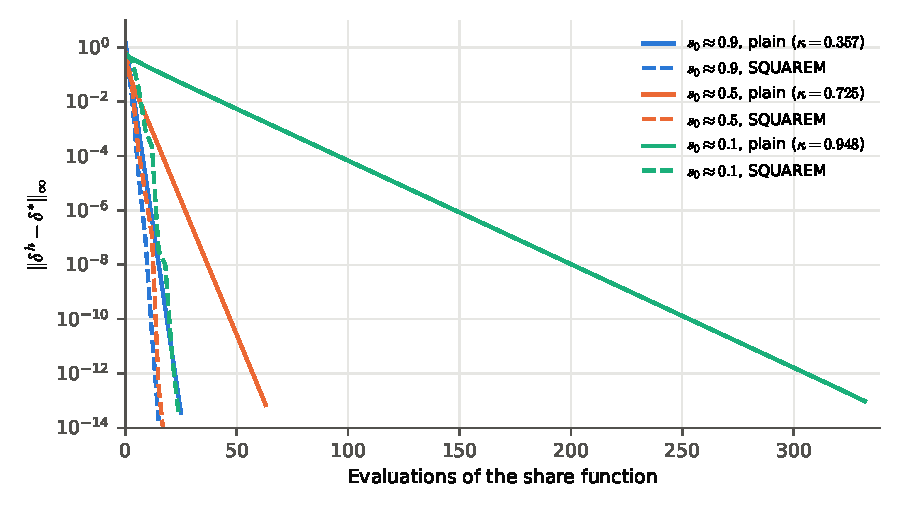
\includegraphics[width=0.92\textwidth]{figures/ch08/fig_contraction.pdf}
  \caption{Convergence of the share inversion in three simulated markets with outside shares near 0.9, 0.5
  and 0.1. Each market has $J = 10$ products, random coefficients with standard deviations
  $(1.0, 1.0, 0.5)$ on the constant, a characteristic and price, and $n_s = 1{,}000$ draws. Solid lines show
  the plain iteration $\delta^{h+1} = \Phi(\delta^h)$. Dashed lines show SQUAREM, the extrapolation method
  described below, on the same map. The
  horizontal axis counts evaluations of the share function. The legend reports the largest row sum $\kappa$
  of the Jacobian of $\Phi$ at the solution. Computed in \texttt{fig\_contraction.py}.}
  \label{fig:08-contraction}
\end{figure}

\subsubsection{Starting values and the multiplicative form}
The logit inversion is the natural first starting value, since it is exact at $\theta_2 = 0$. Inside an
estimation routine the outer optimizer changes $\theta_2$ by small amounts, and the solution at the previous
trial value is a better start. This warm start can cut the number of iterations considerably. Exponentiating
the update gives the equivalent form
\begin{equation*}
  e^{\delta^{h+1}_{jt}} = e^{\delta^h_{jt}}\,\frac{s^{\text{obs}}_{jt}}{s_{jt}(\delta^h_t;\theta_2)},
\end{equation*}
which works with $e^{\delta}$ directly and avoids a logarithm and an exponential per product and iteration.
Each iteration raises $\delta_{jt}$ when the model underpredicts the share of $j$ and lowers it when the model
overpredicts. The individual choice probabilities should be computed with the overflow-safe evaluation of
\cref{sec:08-simulation}.

\subsubsection{The stopping rule}
The iteration stops when successive iterates are close. The next result converts this observable criterion
into a bound on the distance to the solution.

\begin{proposition}[Inner-loop error]\label{prop:08-innererror}
Suppose $\Phi_t$ is a contraction with modulus $\kappa < 1$ on a set that contains the iterates and the
solution $\delta^*_t$. If the iteration stops at the first $H$ with $\Vert \delta^H_t - \delta^{H-1}_t\Vert
\leq \epsilon_{in}$, then
\begin{equation*}
  \Vert \delta^H_t - \delta^*_t \Vert \leq \frac{\kappa}{1 - \kappa}\,\epsilon_{in}.
\end{equation*}
\end{proposition}

\begin{proof}
Since $\delta^*_t = \Phi_t(\delta^*_t)$ and $\delta^H_t = \Phi_t(\delta^{H-1}_t)$,
\begin{align*}
  \Vert \delta^H_t - \delta^*_t\Vert &= \Vert \Phi_t(\delta^{H-1}_t) - \Phi_t(\delta^*_t)\Vert
  \leq \kappa\Vert \delta^{H-1}_t - \delta^*_t\Vert \\
  &\leq \kappa\big(\Vert \delta^{H-1}_t - \delta^{H}_t\Vert + \Vert \delta^H_t - \delta^*_t\Vert\big)
  \leq \kappa\epsilon_{in} + \kappa\Vert \delta^H_t - \delta^*_t\Vert.
\end{align*}
Collecting the terms in $\Vert \delta^H_t - \delta^*_t\Vert$ gives $(1 - \kappa)\Vert \delta^H_t -
\delta^*_t\Vert \leq \kappa\epsilon_{in}$.
\end{proof}

When $\kappa$ is near one, the error can exceed the tolerance by orders of magnitude. In the third market of
\cref{fig:08-contraction} ($\kappa = 0.948$), stopping at a step size of $10^{-4}$ leaves a true error of
$1.0 \times 10^{-3}$, against a bound of $1.7 \times 10^{-3}$. Stopping at $10^{-8}$ leaves $1.0 \times
10^{-7}$. The error is about ten times the tolerance.

The inner error then contaminates the outer problem. Let $e = \tilde\delta - \delta(\theta_2)$ be the
inversion error, stacked over markets. \Cref{sec:08-gmm} shows that the structural error is $\xi(\theta_2) =
\bm{M}\delta(\theta_2)$ for a matrix $\bm{M}$ that does not depend on $\theta_2$ given the weighting matrix.
The computed moments therefore carry the error $\frac{1}{N}\bm{Z}^\T \bm{M} e$. This error varies with
$\theta_2$ in an erratic way, because the number of inner iterations jumps from one trial value to the next.
A finite-difference derivative with step $\Delta$ inherits an error of order $\frac{\Vert e\Vert}{\Delta}$.
With $\Vert e\Vert$ near $10^{-6}$ and $\Delta$ near $10^{-6}$, the error in the computed gradient is of
order one. \citet[Sections~4.2 and~6]{DubeFoxSu2012} show that a loose inner tolerance can keep the outer
optimizer from converging. If the researcher then loosens the outer tolerance, the reported solution may not be a
local minimum. In their synthetic data, no run with inner tolerance $10^{-4}$ and outer tolerance $10^{-6}$
reports convergence (their Table~I). The practical rule is to set the inner
tolerance close to machine precision, for example $10^{-12}$ to $10^{-14}$ in the sup norm, and well below the
outer tolerance. With the warm start this costs little.

\subsubsection{Acceleration}
Two methods speed up the inner loop. The first is SQUAREM, a squared extrapolation method of
\citet{VaradhanRoland2008} designed for slowly converging fixed point iterations.
\citet[Section~2.3]{ReynaertsVaradhanNash2012} apply it to the BLP map. One cycle of the variant we use computes
two plain steps, extrapolates and ends with one more plain step \citep[Table~1]{VaradhanRoland2008}. The step
length $a$ is that of their scheme SqS3, set to $-1$ whenever it exceeds $-1$ (their eqs.~(9) and~(20) and
Section~6):
\begin{gather*}
  r = \Phi(\delta) - \delta, \qquad v = \Phi(\Phi(\delta)) - 2\Phi(\delta) + \delta, \qquad
  a = \min\Big\{-\frac{\Vert r\Vert_2}{\Vert v\Vert_2},\, -1\Big\}, \\
  \delta' = \delta - 2ar + a^2 v, \qquad \delta^{new} = \Phi(\delta').
\end{gather*}
With $a = -1$ the cycle reduces to three plain steps. A more negative $a$ extrapolates along the direction in
which the iterates have been moving. In \cref{fig:08-contraction} SQUAREM reaches an error of $10^{-13}$ after
15, 18 and 24 evaluations of the share function, against 25, 63 and 332 for the plain iteration. Its advantage
grows with the modulus. The second method applies Newton's method to the system $\ln s_t(\delta_t;\theta_2)
= \ln s^{\text{obs}}_t$:
\begin{equation*}
  \delta^{h+1}_t = \delta^h_t - \Big[\frac{\partial \ln s_t(\delta^h_t;\theta_2)}{\partial
  \delta_t^\T}\Big]^{-1}\big(\ln s_t(\delta^h_t;\theta_2) - \ln s^{\text{obs}}_t\big).
\end{equation*}
The Jacobian is available in closed form from the proof of \cref{cor:08-rowsum}, and it is nonsingular by
\cref{rem:08-berry-proof}. Newton's method converges quadratically near the solution but may overshoot far
from it. A common hybrid runs the contraction first and switches to Newton steps once the iterates are close.

\begin{remark}[Dampening in the random coefficients nested logit]\label{rem:08-rcnl}
When random coefficients are combined with a nested logit error with nesting parameter $\rho \in [0,1)$, the
undampened map need not be a contraction. We write the nesting parameter as $\rho$ in this remark, because
$\sigma$ here denotes the standard deviations of the random coefficients.
\citet[pp.~919 and 934--935]{GrigolonVerboven2014} show for the plain nested logit that dampening the step by the
factor $1 - \rho$ restores BLP's sufficient conditions for a contraction. They state that the argument extends to
random coefficients and use the same dampened map in the random coefficients nested logit. The
dampened iteration is $\delta^{h+1} = \delta^h + (1 - \rho)\big(\ln s^{\text{obs}} - \ln s(\delta^h)\big)$. Their
printed equation~(7) attaches the factor $1 - \rho$ to $\ln s(\delta^h)$ alone. \citet[eq.~15 and n.~20]{ConlonGortmaker2020}
point out this typesetting error. In the plain nested logit, $\delta_j
= (1 - \rho)\ln s_j + \rho\ln s_g - \ln s_0$, where $s_g$ is the share of $j$'s nest. Holding the nest and
outside shares fixed, a change in $\ln s_j$ therefore maps into a change of $1 - \rho$ times as much in
$\delta_j$, and the dampened step has this scale. \Cref{ch:mergers} uses this model for merger simulation.
\end{remark}

\section{The GMM estimator}\label{sec:08-gmm}

With the inversion in hand, estimation follows the logic of instrumental variables. This section derives the
estimator, the shortcut that concentrates out the linear parameters, the algorithm, its gradient, the
weighting matrix, and the asymptotic variance with simulation error. It ends with a reformulation as a
constrained optimization problem.

\subsection{Why the error must be the structural error}\label{sec:08-why-xi}

A direct approach would choose the parameters to make predicted shares close to observed shares,
\begin{equation*}
  \min_{\theta}\ \big\Vert s\big(x, p, \delta(x, p, \xi;\theta_1);\theta_2\big) - s^{\text{obs}}\big\Vert,
\end{equation*}
as in equation (7) of \citet{Nevo2000a}. \Citet[pp.~530--531]{Nevo2000a} gives two reasons against it. First,
all parameters enter nonlinearly, and with many brand and time dummies the nonlinear search becomes costly.
Second, and more fundamentally, the approach cannot handle the correlation between prices and $\xi$. The
residual $s^{\text{obs}} - s(\cdot)$ is a nonlinear function of $\xi$. The standard nonlinear simultaneous equations
model allows parameters and variables to enter nonlinearly, but it requires an additively separable error
\citep[p.~531]{Nevo2000a}. The share residual does not have this form. At the true parameters the
predicted share depends on the unknown vector $\xi$. Setting $\xi = 0$ in the prediction leaves a residual
that is a nonlinear function of $\xi$. An orthogonality condition between instruments and $\xi$ then implies no
such condition for the residual.

\citet{Berry1994} proposed to define the econometric error as the structural error $\xi_{jt}$ itself. The
link to economic theory is then direct, and we can reason about which variables are plausibly uncorrelated
with unobserved quality \citep[p.~531]{Nevo2000a}. The cost is the inversion of \cref{sec:08-inversion}.

\subsection{Moment conditions}\label{sec:08-moments}

The identifying assumption of \citet[eq.~4.1]{BerryLevinsohnPakes1995} is a conditional moment restriction.
Let $\mathcal{Z}_t$ denote the exogenous variables of market $t$: the observed characteristics of all products
and the cost shifters. BLP assume
\begin{equation}\label{eq:08-cond-moment}
  \E[\xi_{jt} \mid \mathcal{Z}_t] = 0 \quad\text{and}\quad \E[\omega_{jt} \mid \mathcal{Z}_t] = 0,
\end{equation}
where $\omega_{jt}$ is the cost unobservable of \cref{sec:08-supply}. Prices and quantities are left out of
the conditioning set because the model makes them functions of $\xi$ and $\omega$. The characteristics are
included because the model does not explain how they are chosen \citep[p.~854]{BerryLevinsohnPakes1995}.
\Cref{sec:08-instruments} discusses how plausible this is. In this section we treat demand alone.

A conditional moment restriction implies that $\xi_{jt}$ is uncorrelated with every function of
$\mathcal{Z}_t$. We choose $L$ such functions and collect them in the row vector $z_{jt} \in \R^{1\times L}$,
the \emph{instruments} for observation $(j,t)$. The unconditional moment conditions are
\begin{equation}\label{eq:08-moments}
  \E\big[z_{jt}^\T\,\xi_{jt}(\theta_0)\big] = 0,
\end{equation}
which is equation (8) of \citet{Nevo2000a}. The structural error as a function of the parameters is
\begin{equation}\label{eq:08-xi-theta}
  \xi_{jt}(\theta) = \delta_{jt}(s^{\text{obs}}_t;\theta_2) - x_{jt}\beta + \alpha p_{jt}
\end{equation}
\citep[eq.~13]{Nevo2000a}. The observed shares enter through the inversion. For a trial $\theta_2$, the
inversion finds the mean utilities that rationalize the data. The error is the gap between those mean
utilities and the ones predicted by the linear parameters $(\alpha, \beta)$. When the specification includes
brand and time dummies, they appear on the right-hand side of \eqref{eq:08-xi-theta} and the error becomes the
market-specific deviation $\tilde\xi_{jt}$ of \cref{sec:08-brand-fe}.

We stack the $N = \sum_t J_t$ observations. Let $\delta(\theta_2)$ be the $N$-vector of inverted mean
utilities, $\bm{X}$ the $N \times K_1$ matrix whose rows are $(x_{jt}, p_{jt})$ augmented with any dummies,
and $\theta_1 = (\beta^\T, -\alpha)^\T$ the corresponding coefficient vector. This is the vector of linear
parameters $(\alpha, \beta)$ of \cref{sec:08-linear}, ordered and signed to match the columns of $\bm{X}$. Then
\begin{equation*}
  \xi(\theta) = \delta(\theta_2) - \bm{X}\theta_1.
\end{equation*}
Let $\bm{Z}$ be the $N \times L$ matrix of instruments. The sample moments and the GMM objective are
\begin{equation}\label{eq:08-gmm-obj}
  g_N(\theta) = \frac{1}{N}\bm{Z}^\T\xi(\theta), \qquad
  Q_N(\theta) = g_N(\theta)^\T W g_N(\theta) = \frac{1}{N^2}\,\xi(\theta)^\T\bm{Z}W\bm{Z}^\T\xi(\theta),
\end{equation}
for a positive definite $L \times L$ weighting matrix $W$. This is equation (9) of \citet{Nevo2000a} and
equation (6) of \citet{Nevo2001}, who write $W$ as the inverse of an estimate of $\E[\bm Z^\T\xi\xi^\T\bm Z]$.
The GMM estimator is $\hat\theta = \argmin_\theta Q_N(\theta)$. The order condition
requires $L \geq K_1 + K_2$, where $K_2 = \dim\theta_2$. The rank condition requires that
$\E[z_{jt}^\T\frac{\partial \xi_{jt}(\theta_0)}{\partial \theta^\T}]$ have full column rank.
\Cref{app:econometrics} reviews the general theory.

\subsection{Concentrating out the linear parameters}\label{sec:08-concentrate}

The objective \eqref{eq:08-gmm-obj} is quadratic in $\theta_1$ for fixed $\theta_2$. The linear parameters
can therefore be solved in closed form \citep[p.~868]{BerryLevinsohnPakes1995}.

\begin{proposition}[Concentrating out $\theta_1$]\label{prop:08-concentrate}
Suppose $\bm{X}^\T\bm{Z}W\bm{Z}^\T\bm{X}$ is nonsingular. For each $\theta_2$, the value of $\theta_1$ that
minimizes $Q_N(\theta_1, \theta_2)$ is
\begin{equation}\label{eq:08-theta1hat}
  \hat\theta_1(\theta_2) = \big(\bm{X}^\T\bm{Z}W\bm{Z}^\T\bm{X}\big)^{-1}\bm{X}^\T\bm{Z}W\bm{Z}^\T\delta(\theta_2).
\end{equation}
The implied structural error is $\xi(\theta_2) = \bm{M}\delta(\theta_2)$ with $\bm{M} = I_N -
\bm{X}(\bm{X}^\T\bm{Z}W\bm{Z}^\T\bm{X})^{-1}\bm{X}^\T\bm{Z}W\bm{Z}^\T$. The GMM estimator of $\theta_2$
minimizes the profiled objective
\begin{equation}\label{eq:08-profiled}
  Q^c_N(\theta_2) = \frac{1}{N^2}\,\delta(\theta_2)^\T\bm{M}^\T\bm{Z}W\bm{Z}^\T\bm{M}\,\delta(\theta_2),
\end{equation}
and $\hat\theta_1 = \hat\theta_1(\hat\theta_2)$.
\end{proposition}

\begin{proof}
Fix $\theta_2$ and write $\delta = \delta(\theta_2)$. The objective is
\begin{equation*}
  Q_N = \frac{1}{N^2}(\delta - \bm{X}\theta_1)^\T\bm{Z}W\bm{Z}^\T(\delta - \bm{X}\theta_1).
\end{equation*}
Its gradient with respect to $\theta_1$ is
\begin{equation*}
  \frac{\partial Q_N}{\partial \theta_1} = -\frac{2}{N^2}\bm{X}^\T\bm{Z}W\bm{Z}^\T(\delta - \bm{X}\theta_1).
\end{equation*}
Setting it to zero gives the normal equations $\bm{X}^\T\bm{Z}W\bm{Z}^\T\bm{X}\,\theta_1 =
\bm{X}^\T\bm{Z}W\bm{Z}^\T\delta$, whose solution is \eqref{eq:08-theta1hat}. The Hessian
$\frac{2}{N^2}\bm{X}^\T\bm{Z}W\bm{Z}^\T\bm{X}$ is positive definite, so this is the unique minimum.
Substituting, $\delta - \bm{X}\hat\theta_1(\theta_2) = \bm{M}\delta$, and the objective at the minimum is
\eqref{eq:08-profiled}. Finally, $\min_{\theta_1,\theta_2}Q_N = \min_{\theta_2}\min_{\theta_1}Q_N =
\min_{\theta_2}Q^c_N(\theta_2)$.
\end{proof}

The matrix $\bm{M}$ depends on the data and on $W$ only. It can be computed once for each weighting matrix,
and each objective evaluation then requires one matrix-vector product. The nonlinear search runs over
$\theta_2$ alone, which typically has a handful of elements. The number of random coefficients therefore drives the
cost of estimation. The mean utility can include many characteristics, and even brand dummies, at little cost
(\cref{sec:08-model}).

\begin{corollary}[Logit and nested logit as 2SLS]\label{cor:08-2sls}
In the logit model $\theta_2$ is empty and $\delta_{jt} = \ln s^{\text{obs}}_{jt} - \ln s^{\text{obs}}_{0t}$. With $W =
(\frac{1}{N}\bm{Z}^\T\bm{Z})^{-1}$, the estimator \eqref{eq:08-theta1hat} is two-stage least squares of
$\ln s_{jt} - \ln s_{0t}$ on $\bm{X}$ with instruments $\bm{Z}$. In the nested logit model the same holds
after adding $\ln s_{j|g,t}$ to $\bm{X}$ as a second endogenous regressor with coefficient $\sigma$.
\end{corollary}

\begin{proof}
Write $P_Z = \bm{Z}(\bm{Z}^\T\bm{Z})^{-1}\bm{Z}^\T$. The scalar $\frac{1}{N}$ in $W$ cancels from
\eqref{eq:08-theta1hat}, which becomes $(\bm{X}^\T P_Z\bm{X})^{-1}\bm{X}^\T P_Z\delta$, the 2SLS formula. In
the nested logit model $\ln s_{jt} - \ln s_{0t} = x_{jt}\beta - \alpha p_{jt} + \sigma\ln s_{j|g,t} +
\xi_{jt}$, which is linear in $(\beta, \alpha, \sigma)$.
\end{proof}

\Citet[p.~533 and n.~22]{Nevo2000a} and \citet[p.~319]{Nevo2001} make the same point. The weighting matrix
$(\bm{Z}^\T\bm{Z})^{-1}$ is efficient when the errors are homoskedastic.

\subsection{The nested fixed point algorithm}\label{sec:08-nfxp}

The estimator nests the inversion (a fixed point problem) inside the minimization. We call the procedure the
\emph{nested fixed point} (NFXP) algorithm. \citet[p.~863]{BerryLevinsohnPakes1995} describe four steps for
each evaluation of the moments. They estimate the market shares by simulation and solve for the demand
unobservables. They then compute the cost unobservables as price minus the markup, and they interact both
unobservables with the instruments. In our notation the algorithm reads as follows.

\begin{enumerate}[label=\arabic*.,leftmargin=2em]
  \item Before the search, draw $(D_i, \nu_i)$, $i = 1, \dots, n_s$, for each market and hold the draws fixed
  for the whole estimation. Choose the first-step weighting matrix $W = (\frac{1}{N}\bm{Z}^\T\bm{Z})^{-1}$ and
  compute $\bm{M}$.
  \item The outer optimizer proposes a value $\theta_2^{(k)}$. Compute $\mu_{ijt} = \tilde x_{jt}(\Pi D_i +
  \Sigma\nu_i)$ for all draws, products and markets.
  \item In each market, iterate $\delta^{h+1}_t = \Phi_t(\delta^h_t)$ from the last solution until $\Vert
  \delta^{h+1}_t - \delta^h_t\Vert_\infty < \epsilon_{in}$, using the simulated share $s^{n_s}_t$ of
  \cref{sec:08-simulation}.
  \item Compute $\hat\theta_1(\theta_2^{(k)})$ by \eqref{eq:08-theta1hat} and $\xi(\theta_2^{(k)}) =
  \bm{M}\delta(\theta_2^{(k)})$. With a supply side, also compute the markups and the cost unobservable
  $\omega$ (\cref{sec:08-supply}).
  \item Evaluate $Q^c_N(\theta_2^{(k)})$ and its gradient (\cref{prop:08-gradient}). Return them to the
  optimizer, which either stops or returns to step 2.
  \item After convergence, compute the second-step weighting matrix from the first-step residuals
  (\cref{sec:08-weighting}) and repeat steps 2 to 5.
\end{enumerate}

\Cref{fig:08-nfxp} displays the algorithm. Two remarks concern the outer search. \citet[p.~868]%
{BerryLevinsohnPakes1995} use the Nelder-Mead simplex method, which needs no derivatives. \citet[p.~319]%
{Nevo2001} uses a quasi-Newton method with an analytic gradient and reports that it ``was found to work much
faster.'' Holding the draws fixed is essential for the outer search. Fresh draws at each evaluation would make
the objective a random function of $\theta_2$, and no optimizer would converge \citep{PakesPollard1989}.

\begin{figure}[htbp]
\centering
\begin{tikzpicture}[
  node distance=5mm,
  box/.style={draw, rounded corners=2pt, align=center, font=\small, text width=7.4cm, inner sep=4pt},
  dec/.style={draw, diamond, aspect=3.2, align=center, font=\small, inner sep=0.5pt},
  note/.style={draw, dashed, rounded corners=2pt, align=left, font=\footnotesize, text width=3.3cm,
    inner sep=3pt},
  arr/.style={-{Stealth[length=2.2mm]}, thick}]
\node[box] (draws) {Draw $(D_i, \nu_i)$, $i = 1, \dots, n_s$, in each market once and hold them fixed.
  Set $W = (\frac{1}{N}\bm{Z}^\T\bm{Z})^{-1}$};
\node[box, below=of draws] (outer) {Outer step: the optimizer proposes $\theta_2^{(k)}$};
\node[box, below=of outer] (mu) {Compute $\mu_{ijt} = \tilde x_{jt}(\Pi D_i + \Sigma\nu_i)$\\ for all $i$, $j$, $t$};
\node[box, below=of mu] (inner) {Inner step in each market:\\ $\delta^{h+1}_t = \delta^{h}_t + \ln s^{\text{obs}}_t
  - \ln s^{n_s}_t(\delta^h_t;\theta_2^{(k)})$};
\node[dec, below=of inner] (tol) {$\Vert\delta^{h+1}_t - \delta^{h}_t\Vert_\infty < \epsilon_{in}$?};
\node[box, below=of tol] (lin) {Concentrate out $\hat\theta_1(\theta_2^{(k)})$\\ and set
  $\xi(\theta_2^{(k)}) = \bm{M}\delta(\theta_2^{(k)})$.\\ With a supply side, also $\omega(\theta^{(k)})$};
\node[box, below=of lin] (obj) {Objective $Q^c_N(\theta_2^{(k)})$ and gradient $\nabla Q^c_N(\theta_2^{(k)})$};
\node[dec, below=of obj] (conv) {Outer stopping rule met?};
\node[box, below=of conv] (done) {Report $\hat\theta_2$ and $\hat\theta_1(\hat\theta_2)$.
  Update $W$ and repeat (second step)};
\draw[arr] (draws) -- (outer);
\draw[arr] (outer) -- (mu);
\draw[arr] (mu) -- (inner);
\draw[arr] (inner) -- (tol);
\draw[arr] (tol) -- node[right, font=\footnotesize] {yes} (lin);
\draw[arr] (tol.east) -| node[above, font=\footnotesize, pos=0.25] {no} ([xshift=6mm]inner.east)
  -- (inner.east);
\draw[arr] (lin) -- (obj);
\draw[arr] (obj) -- (conv);
\draw[arr] (conv) -- node[right, font=\footnotesize] {yes} (done);
\draw[arr] (conv.west) -| node[above, font=\footnotesize, pos=0.25] {no} ([xshift=-6mm]outer.west)
  -- (outer.west);
\node[note, right=1.4cm of inner] {Warm start from the last $\delta_t$. Tolerance near machine precision.
  SQUAREM or Newton steps speed it up};
\node[note, right=1.4cm of obj] {Gradient by \cref{prop:08-gradient}. Optimizer: Nelder-Mead or
  quasi-Newton};
\end{tikzpicture}
\caption{The nested fixed point algorithm. The outer loop searches over the nonlinear parameters
$\theta_2$. For each trial value the inner loop inverts the share equations market by market, the linear
parameters are concentrated out, and the profiled GMM objective is evaluated.}
\label{fig:08-nfxp}
\end{figure}

\subsection{The gradient}\label{sec:08-gradient}

Quasi-Newton methods need the gradient of $Q^c_N$. Because $\delta(\theta_2)$ is defined implicitly by the
share equations, its derivative comes from the implicit function theorem (\cref{app:math}).

\begin{proposition}[Gradient of the profiled objective]\label{prop:08-gradient}
For each market, $\delta_t(\theta_2)$ is continuously differentiable and
\begin{equation}\label{eq:08-ift}
  \frac{\partial \delta_t}{\partial \theta_2^\T} = -\Big[\frac{\partial s_t}{\partial
  \delta_t^\T}\Big]^{-1}\frac{\partial s_t}{\partial \theta_2^\T}.
\end{equation}
In the random coefficients logit model with diagonal $\Sigma = \diag(\sigma_1, \dots, \sigma_{K+1})$ and
demographic coefficients $\pi_{kd}$, the derivatives on the right are
\begin{align}
  \frac{\partial s_{jt}}{\partial \delta_{kt}} &= \int s_{ijt}\big(\indic\{j = k\} - s_{ikt}\big)\, \dd F,
  \notag\\
  \frac{\partial s_{jt}}{\partial \sigma_k} &= \int s_{ijt}\,\nu_{ik}\Big(\tilde x_{jtk} - \sum_{m \in
  \mathcal{J}_t}s_{imt}\tilde x_{mtk}\Big)\, \dd F, \label{eq:08-dsdsigma}\\
  \frac{\partial s_{jt}}{\partial \pi_{kd}} &= \int s_{ijt}\,D_{id}\Big(\tilde x_{jtk} - \sum_{m \in
  \mathcal{J}_t}s_{imt}\tilde x_{mtk}\Big)\, \dd F. \notag
\end{align}
The gradient of the profiled objective is
\begin{equation}\label{eq:08-grad}
  \nabla Q^c_N(\theta_2) = \frac{2}{N^2}\Big(\frac{\partial \delta}{\partial \theta_2^\T}\Big)^\T
  \bm{Z}W\bm{Z}^\T\xi(\theta_2).
\end{equation}
\end{proposition}

\begin{proof}
The inverted mean utilities satisfy the identity $s_t(\delta_t(\theta_2);\theta_2) = s^{\text{obs}}_t$ for all
$\theta_2$. Differentiating with respect to $\theta_2^\T$ gives
\begin{equation*}
  \frac{\partial s_t}{\partial \delta_t^\T}\,\frac{\partial \delta_t}{\partial \theta_2^\T} +
  \frac{\partial s_t}{\partial \theta_2^\T} = 0.
\end{equation*}
The Jacobian $\frac{\partial s_t}{\partial \delta_t^\T}$ is nonsingular by \cref{rem:08-berry-proof}, so the
implicit function theorem applies and yields \eqref{eq:08-ift}. The derivative with respect to $\delta$ was
computed in the proof of \cref{cor:08-rowsum}. For $\sigma_k$, note that $\mu_{ijt} = \sum_k \tilde
x_{jtk}(\sigma_k\nu_{ik} + \sum_d \pi_{kd}D_{id})$, so $\frac{\partial \mu_{ijt}}{\partial \sigma_k} = \tilde
x_{jtk}\nu_{ik}$. From $\ln s_{ijt} = \delta_{jt} + \mu_{ijt} - \ln(1 + \sum_m e^{\delta_{mt} + \mu_{imt}})$,
\begin{equation*}
  \frac{\partial \ln s_{ijt}}{\partial \sigma_k} = \tilde x_{jtk}\nu_{ik} - \sum_m s_{imt}\tilde
  x_{mtk}\nu_{ik},
\end{equation*}
and multiplying by $s_{ijt}$ and integrating gives \eqref{eq:08-dsdsigma}. The derivative with respect to
$\pi_{kd}$ replaces $\nu_{ik}$ by $D_{id}$. For the gradient, write $Q_N(\theta_1, \theta_2)$ as in
\eqref{eq:08-gmm-obj}, so $Q^c_N(\theta_2) = Q_N(\hat\theta_1(\theta_2), \theta_2)$. By the chain rule,
\begin{equation*}
  \nabla Q^c_N = \frac{\partial Q_N}{\partial \theta_2} + \Big(\frac{\partial \hat\theta_1}{\partial
  \theta_2^\T}\Big)^\T\frac{\partial Q_N}{\partial \theta_1}.
\end{equation*}
The second term vanishes because $\frac{\partial Q_N}{\partial \theta_1} = 0$ at $\hat\theta_1(\theta_2)$.
This is the envelope theorem. Holding $\theta_1$ fixed, $\frac{\partial \xi}{\partial \theta_2^\T} =
\frac{\partial \delta}{\partial \theta_2^\T}$, which gives \eqref{eq:08-grad}.
\end{proof}

With simulation, every integral in the proposition is replaced by the average over the $n_s$ fixed draws.
The gradient then costs about as much as one more share evaluation plus the solution of a $J_t \times J_t$
linear system in each market. The matrix $\frac{\partial \delta}{\partial \theta_2^\T}$ also reappears in the
asymptotic variance below and in the optimal instruments of \cref{sec:08-optiv}.

\subsection{Weighting, efficiency and clustering}\label{sec:08-weighting}

The efficient weighting matrix is the inverse of the variance of the moments. With independent observations
the second-step matrix is
\begin{equation*}
  W_2 = \Big[\frac{1}{N}\sum_t\sum_{j \in \mathcal{J}_t} z_{jt}^\T\,\hat\xi_{jt}^2\, z_{jt}\Big]^{-1},
\end{equation*}
where $\hat\xi_{jt}$ are the residuals at the first-step estimate. \citet[p.~319]{Nevo2001} follows this
two-step procedure. He also iterated further and found that ``the estimated parameters changed only slightly
beyond the second iteration.''

Errors are often correlated within groups of observations. \citet[pp.~862--863]{BerryLevinsohnPakes1995}
follow car models over the years they are sold, and the unobservables of one model are more alike across years
than across models. They sum the moments of each model over its years,
\begin{equation*}
  g_m(\theta) = \sum_t \big[f_{mt}(\mathcal{Z})^\T \otimes I_2\big]
  \begin{pmatrix}\xi_{mt}(\theta)\\ \omega_{mt}(\theta)\end{pmatrix},
\end{equation*}
where $f_{mt}(\mathcal{Z})$ is the vector of instrument functions for model $m$ in year $t$ and $\otimes$ is
the Kronecker product. They then minimize a quadratic form in the average of $g_m$ over models. The
resulting standard errors allow arbitrary correlation across years for a given model and arbitrary
heteroskedasticity across models. The corresponding efficient weighting matrix is the inverse of $\frac{1}{M}
\sum_m g_m(\hat\theta)g_m(\hat\theta)^\T$, with $M$ the number of models. The same construction applies with
cities, markets or brands as clusters (\cref{app:econometrics}).

With the efficient weighting matrix, $N\,Q_N(\hat\theta)$ is the \emph{Hansen J statistic}. Under correct
specification it converges in distribution to a $\chi^2$ with $L - K_1 - K_2$ degrees of freedom. A rejection
signals that some instruments are invalid or that the model is misspecified. With tens of thousands of
observations the test rejects almost any model, as \citet[p.~325, n.~23]{Nevo2001} notes.

\subsection{Asymptotic distribution and simulation error}\label{sec:08-asymptotics}

The estimator departs from textbook GMM in two ways. The moments are computed from sampled shares, and the
share integral is simulated. \citet[Section 5]{BerryLevinsohnPakes1995} account for both. Their setting is a
single cross section of $J$ products, with asymptotics as $J$ grows. Let $s^0$ be the population shares,
$s^n$ the shares observed in a sample of $n$ consumers, $P_0$ the distribution of consumer attributes, and
$P_{n_s}$ the empirical distribution of $n_s$ simulation draws. BLP standardize the two unobservables by a
$2 \times 2$ matrix $T(z_j)$ with $T(z_j)^\T T(z_j) = \Upsilon(z_j)^{-1}$, where $\Upsilon(z_j) =
\E[(\xi_j, \omega_j)^\T(\xi_j, \omega_j) \mid z_j]$ (their eqs.~5.1--5.2). BLP write $\Omega$ for this covariance matrix. We write $\Upsilon$ because $\Omega$ is the ownership matrix in this book. They interact the standardized
errors with an $L \times 2$ instrument matrix $H_j(\mathcal Z)$ and form
\begin{equation*}
  G_J(\theta; s, P) = \frac{1}{J}\sum_{j=1}^{J}H_j(\mathcal{Z})\,T(z_j)\begin{pmatrix}\xi_j(\theta, s,
  P)\\ \omega_j(\theta, s, P)\end{pmatrix}
\end{equation*}
(eq.~5.4). The estimator minimizes $\Vert G_J(\theta; s^n, P_{n_s})\Vert$ with $\Vert y\Vert = y^\T y$
(eq.~5.5).

The computed moments differ from the ideal ones $G_J(\theta_0; s^0, P_0)$ in two ways. Adding and subtracting
gives the decomposition
\begin{multline*}
  G_J(\theta_0; s^n, P_{n_s}) = \underbrace{G_J(\theta_0; s^0, P_0)}_{\text{product draws}}
  + \underbrace{\big[G_J(\theta_0; s^n, P_0) - G_J(\theta_0; s^0, P_0)\big]}_{\text{consumer sampling}}\\
  + \underbrace{\big[G_J(\theta_0; s^n, P_{n_s}) - G_J(\theta_0; s^n, P_0)\big]}_{\text{simulation}}.
\end{multline*}
The three terms come from three independent random processes: the draws of the product characteristics
$(x, w, \xi, \omega)$, the sampling of consumers, and the simulation draws. Their variances, scaled by $J$,
converge to
\begin{align*}
  V_1 &= \lim_{J\to\infty}\E_{\mathcal Z}\Big[H_j T(z_j)\begin{pmatrix}\xi_j\\ \omega_j\end{pmatrix}
  \begin{pmatrix}\xi_j\\ \omega_j\end{pmatrix}^\T T(z_j)^\T H_j^\T\Big],\\
  V_2 &= \lim_{J\to\infty}\frac{J}{n}\,\E\Big(n\big[G_J(\theta_0; s^0, P_0) - G_J(\theta_0; s^n,
  P_0)\big]\big[\cdot\big]^\T\Big),\\
  V_3 &= \lim_{J\to\infty}\frac{J}{n_s}\,\E\Big(n_s\big[G_J(\theta_0; s^n, P_{n_s}) - G_J(\theta_0; s^n,
  P_0)\big]\big[\cdot\big]^\T \,\Big|\, s^n\Big),
\end{align*}
where $[\cdot]$ repeats the preceding bracket. The usual GMM linearization then applies. The first-order
condition $\hat G^\T G_J(\hat\theta) = 0$, with $\hat G$ the Jacobian of the moments, and a mean value expansion
$G_J(\hat\theta) \approx G_J(\theta_0) + G(\hat\theta - \theta_0)$ give $\sqrt{J}(\hat\theta - \theta_0)
\approx -(G^\T G)^{-1}G^\T\sqrt{J}\,G_J(\theta_0)$. Hence the asymptotic variance is
\begin{equation}\label{eq:08-blp-avar}
  (G^\T G)^{-1}G^\T(V_1 + V_2 + V_3)\,G\,(G^\T G)^{-1}, \qquad G = \lim_{J\to\infty}\frac{\partial
  \E[G_J(\theta, s^0, P_0)]}{\partial \theta^\T}\Big|_{\theta = \theta_0},
\end{equation}
which is equation (5.6) of \citet{BerryLevinsohnPakes1995}, who write $\Gamma$ for $G$. With a general
weighting matrix the formula becomes $(G^\T WG)^{-1}G^\T W(V_1 + V_2 + V_3)WG(G^\T WG)^{-1}$.

The scale factors explain which terms matter. $V_2$ carries the factor $\frac{J}{n}$, and BLP note that $n$,
the number of U.S. households, ``is on the order of 100 million,'' so $V_2$ is negligible
\citep[p.~859]{BerryLevinsohnPakes1995}. $V_3$ carries the factor $\frac{J}{n_s}$, and with a feasible number
of draws it is not negligible. The limit theory requires $n$ and $n_s$ to grow ``on the order of $J^3$''
(p.~859). The ``in process'' paper that BLP cite for these results was published as
\citet{BerryLintonPakes2004}. Its theorems need the number of draws to grow only at rate $J^2$ in
logit-style models, a weaker condition than the rate BLP quote (\cref{sec:08-pcm}). BLP estimate $V_1$ by its sample analog at $\hat\theta$. They estimate $V_3$ by
drawing new sets of simulation draws, recomputing the moments at $\hat\theta$ for each set, and taking the
empirical variance. The correction ``increases our reported standard errors \dots by about 5--20\% (with the
exception of one parameter, whose reported standard error doubles)'' (p.~859).

The sampling scheme behind $V_1$ deserves a word. BLP do not assume that products are independent draws. They
assume that the vectors $y_j = (\xi_j, \omega_j, z_j)$ are \emph{exchangeable}: their joint density is
unchanged by any permutation of the product labels \citep[p.~856, n.~14]{BerryLevinsohnPakes1995}. This
allows characteristics chosen by firms to be related across products and allows common shocks to many
products.

In data with many markets and a fixed set of products, as in \citet{Nevo2001}, the asymptotics run over
markets instead. The moments are averages of independent market-level terms, and the usual cluster-robust
GMM formulas apply. \citet[p.~319]{Nevo2001} corrects for simulation error by accounting for the fact that
the draws are common to all observations in a market. One caveat carries over from \cref{sec:08-simulation}.
The log of a simulated share is biased (\cref{prop:08-simbias}), so the inverted $\delta$ carries a bias of
order $\frac{1}{n_s}$ that does not average out across markets. Consistency therefore requires $n_s$ to grow
with the sample, and in practice $n_s$ should be large enough that the bias is small relative to the standard
errors.

Two practical points complete the picture. First, the standard errors must be computed for the full
parameter vector $\theta = (\theta_1, \theta_2)$. The moment Jacobian is
\begin{equation*}
  G = \frac{1}{N}\bm{Z}^\T\Big[-\bm{X},\ \frac{\partial \delta}{\partial \theta_2^\T}\Big],
\end{equation*}
with the second block from \cref{prop:08-gradient}. Treating the second-stage regression
\eqref{eq:08-theta1hat} as ordinary 2SLS with $\delta$ as data ignores the estimation of $\theta_2$ and
understates the uncertainty in $\hat\theta_1$. Second, objects such as elasticities, markups and welfare are
nonlinear functions $\varphi(\theta)$. Their uncertainty can be computed by the delta method,
$\widehat{\Var}(\varphi(\hat\theta)) = \nabla\varphi^\T\widehat{\Var}(\hat\theta)\nabla\varphi$, or by a
parametric bootstrap. The bootstrap draws $\theta^{(r)}$ from the estimated asymptotic distribution of
$\hat\theta$, computes $\varphi(\theta^{(r)})$ for each draw, and reads off percentiles.
\citet[pp.~319, 333]{Nevo2001} uses the bootstrap, with 1,500 draws for the margins of his Table VIII
(\cref{sec:08-nevo01}).

\subsection{MPEC: estimation as constrained optimization}\label{sec:08-mpec}

\citet{SuJudd2012} propose to estimate structural models by \emph{mathematical programming with equilibrium
constraints} (MPEC), and \citet{DubeFoxSu2012} apply the idea to BLP. Instead of solving the share equations
for every trial value of $\theta_2$, MPEC treats the mean utilities as additional unknowns and imposes the
share equations as constraints:
\begin{equation}\label{eq:08-mpec}
  \min_{\theta_1, \theta_2, \delta, \eta}\ \eta^\T W\eta \quad\text{subject to}\quad
  s_t(\delta_t;\theta_2) = s^{\text{obs}}_t \ \ (t = 1, \dots, T), \qquad
  \eta = \frac{1}{N}\bm{Z}^\T(\delta - \bm{X}\theta_1).
\end{equation}
The auxiliary vector $\eta \in \R^L$ holds the sample moments.

\begin{proposition}[Equivalence of MPEC and NFXP]\label{prop:08-mpec}
Suppose the conditions of \cref{thm:08-berry94} hold for every $\theta_2$ in the parameter space. Then
$(\hat\theta_1, \hat\theta_2)$ minimizes the GMM objective \eqref{eq:08-gmm-obj} if and only if there exist
$\hat\delta$ and $\hat\eta$ such that $(\hat\theta_1, \hat\theta_2, \hat\delta, \hat\eta)$ solves
\eqref{eq:08-mpec}. In that case $\hat\delta = \delta(\hat\theta_2)$ and $\hat\eta = g_N(\hat\theta)$.
\end{proposition}

\begin{proof}
By \cref{thm:08-berry94}, for each $\theta_2$ the share constraints have exactly one solution,
$\delta(\theta_2)$. The second constraint then determines $\eta$. The feasible set of \eqref{eq:08-mpec} is
therefore
\begin{equation*}
  \Big\{\big(\theta_1, \theta_2, \delta(\theta_2), \frac{1}{N}\bm{Z}^\T(\delta(\theta_2) -
  \bm{X}\theta_1)\big): (\theta_1, \theta_2) \text{ in the parameter space}\Big\}.
\end{equation*}
On this set the objective equals $g_N(\theta)^\T Wg_N(\theta) = Q_N(\theta)$. Minimizing over the feasible set
is the same as minimizing $Q_N$ over $\theta$, and the minimizers correspond one to one. The map
$\theta_2 \mapsto \delta(\theta_2)$ is continuous by \cref{prop:08-gradient}, so local minimizers also
correspond.
\end{proof}

The two formulations have the same solutions and different computational properties. MPEC has no inner loop,
so there is no inner tolerance and no propagation of inversion error into the objective. The share
constraints need hold only at the solution, so the solver does not spend effort on precise inversions at trial
values far from the optimum. The constraint Jacobian is sparse, because $s_t$ depends only on $\delta_t$ and
$\theta_2$. Derivatives can be supplied by automatic differentiation. Against this, the problem has $K_1 +
K_2 + N + L$ unknowns, $N$ nonlinear share constraints and $L$ linear moment constraints. It requires a large-scale constrained solver and
careful scaling, and the solver may stop at an infeasible point. \citet[Section~7]{DubeFoxSu2012} find MPEC
faster than NFXP when the contraction is slow. By \cref{cor:08-rowsum}, this happens when outside shares are
small. With an outside share of 0.35 in their experiments, MPEC is about 24 times faster (their Table~III).
\citet[Sections~3 and~5]{ConlonGortmaker2020} instead use the nested fixed point. They prefer an inner tolerance
between $10^{-14}$ and $10^{-12}$. They find SQUAREM the fastest and most reliable way to accelerate the
contraction.
The choice between the two is a matter of implementation. The statistical properties of the estimator are the same.

Other estimators trade exactness for speed. \citet[Section~5]{LeeSeo2015} linearize the log share function around
the current mean utilities and invert this approximation analytically at each trial value. After each minimization
they update the point of approximation by one Newton step. The share equations therefore hold exactly only at the
optimum.
\citet[Sections~2 and~3]{SalanieWolak2019} expand the inverse share function to second order around zero random
coefficients. The resulting approximate model is linear in the mean coefficients and in the variances and
covariances of the random coefficients. Two-stage least squares therefore estimates it. These estimates can serve as
starting values for the exact estimator.
\Cref{prop:08-smallsigma} below derives the leading term of such an expansion.

\section{Instruments and identification}\label{sec:08-instruments}

The estimator of \cref{sec:08-gmm} is only as good as its instruments. This section first explains why prices
need instruments, how many instruments are needed and which roles they play. It then derives the efficient
instruments and reviews the instrument families used in practice. It closes with brand fixed effects and with
nonparametric identification.

\subsection{Price endogeneity}\label{sec:08-endogeneity}

Firms observe $\xi_{jt}$ when they set prices. In a Nash-Bertrand equilibrium the price is marginal cost
plus a markup (\cref{ch:diffprod}), and the markup depends on demand, hence on $\xi_t$. \citet[eq.~8]%
{Nevo2001} writes
\begin{equation*}
  p_{jt} = mc_{jt} + f(\xi_{jt}, \dots) = (mc_j + f_j) + \big(mc_{jt} - mc_j + f_{jt} - f_j\big),
\end{equation*}
where $mc_j$ and $f_j$ are brand means and the second bracket is the deviation of the market from them. With
brand dummies the brand means are absorbed, but the market-specific deviation of the markup still moves with
the market-specific deviation of $\xi$ \citep[p.~320]{Nevo2001}.

A single-product logit firm makes the sign transparent. Its first-order condition gives the markup $m_j =
p_j - mc_j = \frac{1}{\alpha(1 - s_j)}$ (\cref{ch:logit}). Hold rivals' prices fixed and define
\begin{equation*}
  G(m_j, \xi_j) = m_j - \frac{1}{\alpha\big(1 - s_j(m_j, \xi_j)\big)},
\end{equation*}
where $s_j$ is the logit share at price $mc_j + m_j$. The optimal markup solves $G(m_j, \xi_j) = 0$. The logit
derivatives are $\frac{\partial s_j}{\partial m_j} = -\alpha s_j(1 - s_j)$ and $\frac{\partial s_j}{\partial
\xi_j} = s_j(1 - s_j)$. By the chain rule,
\begin{align*}
  \frac{\partial}{\partial m_j}\,\frac{1}{\alpha(1 - s_j)} &= \frac{1}{\alpha(1 - s_j)^2}\,\frac{\partial
  s_j}{\partial m_j} = -\frac{s_j}{1 - s_j},\\
  \frac{\partial}{\partial \xi_j}\,\frac{1}{\alpha(1 - s_j)} &= \frac{1}{\alpha(1 - s_j)^2}\,\frac{\partial
  s_j}{\partial \xi_j} = \frac{s_j}{\alpha(1 - s_j)}.
\end{align*}
Hence
\begin{equation*}
  \frac{\partial G}{\partial m_j} = 1 + \frac{s_j}{1 - s_j} = \frac{1}{1 - s_j}, \qquad
  \frac{\partial G}{\partial \xi_j} = -\frac{s_j}{\alpha(1 - s_j)}.
\end{equation*}
The implicit function theorem then gives the response of the best-response markup to unobserved quality,
\begin{equation*}
  \frac{\partial m_j}{\partial \xi_j} = -\frac{\partial G}{\partial \xi_j}\Big(\frac{\partial G}{\partial
  m_j}\Big)^{-1} = \frac{s_j}{\alpha(1 - s_j)}\,(1 - s_j) = \frac{s_j}{\alpha} > 0.
\end{equation*}
A better unobserved product sells more and carries a higher markup, so $\Cov(p_{jt}, \xi_{jt}) > 0$.

Consider the logit estimating equation $\ln s_{jt} - \ln s_{0t} = x_{jt}\beta - \alpha p_{jt} + \xi_{jt}$
and let $\tilde p_{jt}$ be the residual from projecting $p_{jt}$ on $x_{jt}$. By the Frisch-Waugh theorem the
OLS coefficient on price satisfies
\begin{equation*}
  \plim\, \widehat{(-\alpha)}_{OLS} = -\alpha + \frac{\Cov(\tilde p_{jt}, \xi_{jt})}{\Var(\tilde p_{jt})}
  > -\alpha,
\end{equation*}
when $x_{jt}$ is uncorrelated with $\xi_{jt}$. The estimated price coefficient is biased toward zero, and
demand looks too inelastic. Random coefficients do not remove the problem, since $\xi_{jt}$ enters
$\delta_{jt}$ in the same way.

The evidence matches the theory. In the automobile data of \citet[Table III]{BerryLevinsohnPakes1995}, the
OLS logit price coefficient is $-0.089$ (0.004). It implies that 1,494 of the 2,217 models have inelastic
demand, which is inconsistent with profit maximization. With instruments the coefficient becomes $-0.216$
(0.123), and only 22 models have inelastic demand (pp.~873--874). In the cereal data of \citet[Table V]%
{Nevo2001}, the OLS logit coefficient with brand dummies is $-7.26$ (0.16). The same specification
instrumented with prices in other cities gives $-17.57$ (0.50) (columns ii and v). \Cref{sec:08-blp95,sec:08-nevo01} present these tables in
full.

\subsection{How many instruments, and what they must do}\label{sec:08-iv-roles}

The order condition of \cref{sec:08-moments} counts the instruments. The exogenous characteristics in
$x_{jt}$ serve as their own instruments. The remaining instruments must be at least as many as the
endogenous variables in the mean utility (usually price alone) plus the number of nonlinear parameters. A
model with one random coefficient per characteristic and on price needs $K + 2$ excluded instruments,
where $K$ is the number of characteristics: one for price and $K + 1$ for $\Sigma$.

The instruments play two distinct roles. Some must shift prices, as in any demand system. Others must shift
what \citet[Section 7]{BerryHaile2014} call ``quantities,'' the market shares that enter the inverse demand
function. \citet[p.~1136, n.~2]{BerryHaile2024} note that instruments for quantities are what the applied
literature informally calls instruments for the ``nonlinear parameters.'' The next result shows concretely why
the nonlinear parameters need their own source of variation.

\begin{proposition}[Small-$\sigma$ expansion of the inverse]\label{prop:08-smallsigma}
Suppose there is a single random coefficient, $\mu_{ijt} = \sigma\nu_i x_{jt}$, with $\nu_i$ symmetric
about zero, $\E[\nu_i^2] = 1$ and $\E[e^{c|\nu_i|}] < \infty$ for all $c > 0$, as for the standard normal. Normalize $x_{0t} = 0$ for the outside good and let
$\bar x_t = \sum_{m=0}^{J_t} s_{mt}x_{mt}$ be the share-weighted mean of the characteristic. Then the inverted
mean utility satisfies
\begin{equation*}
  \delta_{jt}(s_t;\sigma) = \ln\frac{s_{jt}}{s_{0t}} - \frac{\sigma^2}{2}\,x_{jt}\big(x_{jt} - 2\bar x_t\big)
  + O(\sigma^4).
\end{equation*}
\end{proposition}

\begin{proof}
Drop $t$. Let $K(\tau) = \ln\sum_{m=0}^{J}e^{\delta_m + \tau x_m}$ with $\delta_0 = 0$. For a consumer with
$\tau = \sigma\nu_i$, $\ln s_{ij} = \delta_j + \tau x_j - K(\tau)$. The function $K$ is the cumulant generating
function of $x$ under the logit probabilities $s^L_m(\delta) = e^{\delta_m - K(0)}$. Hence $K'(0) = \sum_m
s^L_m x_m \equiv \bar x^L$ and $K''(0) = \sum_m s^L_m x_m^2 - (\bar x^L)^2 \equiv V^L$. A second-order
expansion gives
\begin{equation*}
  \ln s_{ij} - \ln s^L_j = \tau(x_j - \bar x^L) - \frac{\tau^2}{2}V^L + O(\tau^3).
\end{equation*}
Exponentiating,
\begin{equation*}
  \frac{s_{ij}}{s^L_j} = 1 + \tau(x_j - \bar x^L) + \frac{\tau^2}{2}\big[(x_j - \bar x^L)^2 - V^L\big] +
  c_j\tau^3 + R_{ij},
\end{equation*}
for a constant $c_j$ and a remainder bounded by $C\tau^4e^{C|\tau|}$ for some constant $C$. Integrating over
$\nu_i$ removes the linear and cubic terms, because $\nu_i$ is symmetric, and $\E[\tau^2] = \sigma^2$. The
moment condition on $\nu_i$ makes the expected remainder of order $\sigma^4$. So
\begin{equation*}
  \ln s_j = \ln s^L_j + \frac{\sigma^2}{2}\big[(x_j - \bar x^L)^2 - V^L\big] + O(\sigma^4), \qquad
  j = 0, 1, \dots, J.
\end{equation*}
Subtract the equation for $j = 0$, where $x_0 = 0$, and use $\ln s^L_j - \ln s^L_0 = \delta_j$:
\begin{equation*}
  \ln\frac{s_j}{s_0} = \delta_j + \frac{\sigma^2}{2}\big[(x_j - \bar x^L)^2 - (\bar x^L)^2\big] + O(\sigma^4)
  = \delta_j + \frac{\sigma^2}{2}x_j(x_j - 2\bar x^L) + O(\sigma^4).
\end{equation*}
Finally, the logit shares differ from the true shares by $O(\sigma^2)$, so replacing $\bar x^L$ by $\bar x$
changes the right-hand side by $O(\sigma^4)$. Solving for $\delta_j$ gives the result.
\end{proof}

We checked the expansion numerically in a market with four products. Their shares are 0.20, 0.15, 0.10 and
0.05, and their characteristic values are 0.5, 1.0, 1.5 and 2.5. At $\sigma = 0.1$ the exact inverse differs from the logit
inversion by up to $1.8 \times 10^{-2}$. It differs from the approximation by at most $8.3 \times 10^{-5}$. The
ratio of this error to $\sigma^4$ stays near 0.8 as $\sigma$ falls from 0.4 to 0.05.

Substituting the expansion into \eqref{eq:08-xi-theta} gives, to second order,
\begin{equation*}
  \xi_{jt}(\theta) \approx \ln\frac{s_{jt}}{s_{0t}} - x_{jt}\beta + \alpha p_{jt} - \frac{\sigma^2}{2}\,
  x_{jt}\big(x_{jt} - 2\bar x_t\big).
\end{equation*}
The parameter $\sigma^2$ multiplies a constructed regressor that depends on the shares through $\bar x_t$.
Shares respond to $\xi$, so this regressor is endogenous, and estimating $\sigma$ requires an instrument that
predicts it, and predicts it separately from price. A cost shifter can do this in principle, because it moves
shares and hence $\bar x_t$. In practice its variation in the constructed regressor is often weak relative to its
variation in price, so identification of $\sigma$ through cost shifters alone tends to be fragile. Natural candidates
are functions of the characteristics of the other products in the market, which shift $\bar x_t$ directly. The regressor also involves the
squared distance of $x_{jt}$ from the market average. This is the logic behind the differentiation instruments
of \cref{sec:08-iv-families}.

\citet[pp.~529--530]{Nevo2000a} gives the economic intuition. Suppose products A and B have similar
characteristics, products B and C have equal shares, and the price of A rises. The logit predicts equal share
gains for B and C, while the random coefficients model allows B to gain more. The observed relative change in
the shares of B and C distinguishes the models, and its size identifies the parameters of the taste
distribution. Data from more markets help, especially when products enter, exit or change characteristics.
Choice-set variation of this kind helps identify the variance of the random tastes. \citet[p.~541]{Nevo2000a}
and \citet[p.~330, n.~27]{Nevo2001} point to its absence in their data to explain imprecise estimates of
$\Sigma$. Identifying the coefficients on demographics, $\Pi$, requires markets with different distributions
of demographics \citep[p.~529]{Nevo2000a}.

\citet[p.~877]{BerryLevinsohnPakes1995} explain why the mean and the variance of a taste are separately
identified. A high mean taste for horsepower and a high variance both raise the share of powerful cars.
The two explanations differ in substitution. With zero variance, consumers who leave a powerful car after a
price increase do not favor other powerful cars. With a large variance, the consumers who leave are those who
value horsepower most, and they move disproportionately to other powerful cars. BLP add that they ``had much
more difficulty estimating separate mean and variance terms from a single cross section'' than from the panel
(n.~30).

\subsection{Optimal instruments}\label{sec:08-optiv}

The conditional moment restriction \eqref{eq:08-cond-moment} makes every function of $\mathcal{Z}_t$ a valid
instrument. Some functions are more informative than others. \citet{Chamberlain1987} characterizes the best
choice.\footnote{\citet{BerryLevinsohnPakes1995} cite this paper as Chamberlain (1986), \emph{Journal of
Econometrics} 33. It appeared in volume 34 in 1987.} Consider a scalar residual with $\E[\xi(\theta_0)
\mid \mathcal{Z}] = 0$ and conditional variance $\varkappa^2(\mathcal{Z})$, and let
\begin{equation*}
  \mathcal{D}(\mathcal{Z}) = \E\Big[\frac{\partial \xi(\theta_0)}{\partial \theta} \,\Big|\, \mathcal{Z}\Big]
\end{equation*}
be the expected derivative of the residual, a column vector of dimension $\dim\theta$.

\begin{proposition}[Optimal instruments]\label{prop:08-optiv}
Consider GMM estimators based on exactly identifying moments $\E[h(\mathcal{Z})\xi(\theta)] = 0$, where
$h$ has dimension $\dim\theta$. Their asymptotic variance is
\begin{equation*}
  \big(\E[h\mathcal{D}^\T]\big)^{-1}\,\E[hh^\T\varkappa^2]\,\big(\E[\mathcal{D}h^\T]\big)^{-1}.
\end{equation*}
It is minimized by $h^*(\mathcal{Z}) = \frac{\mathcal{D}(\mathcal{Z})}{\varkappa^2(\mathcal{Z})}$, and the
minimal variance is $\big(\E[\mathcal{D}\mathcal{D}^\T\varkappa^{-2}]\big)^{-1}$.
\end{proposition}

\begin{proof}
Define $u = h\varkappa$ and $v = \frac{\mathcal{D}}{\varkappa}$. Then $\E[h\mathcal{D}^\T] = \E[uv^\T]$ and
$\E[hh^\T\varkappa^2] = \E[uu^\T]$. We must show
\begin{equation*}
  \E[uv^\T]^{-1}\E[uu^\T]\E[vu^\T]^{-1} - \E[vv^\T]^{-1} \succeq 0.
\end{equation*}
This is equivalent to $\E[vv^\T] - \E[vu^\T]\E[uu^\T]^{-1}\E[uv^\T] \succeq 0$, by taking inverses of both
sides of the inequality between positive definite matrices. Let $\Gamma = \E[vu^\T]\E[uu^\T]^{-1}$. The left
side equals $\E[(v - \Gamma u)(v - \Gamma u)^\T]$, the second moment of a projection residual, which is
positive semidefinite. Equality holds when $u$ is proportional to $v$, that is, when $h \propto
\frac{\mathcal{D}}{\varkappa^2}$.
\end{proof}

For BLP, \citet[eq.~5.7]{BerryLevinsohnPakes1995} write the optimal instruments for the standardized demand
and cost errors as
\begin{equation*}
  H_j(\mathcal{Z}) = \E\Big[\frac{\partial \xi_j(\theta_0, s^0, P_0)}{\partial \theta},\ \frac{\partial
  \omega_j(\theta_0, s^0, P_0)}{\partial \theta} \,\Big|\, \mathcal{Z}\Big]\,T(z_j) \equiv
  \mathcal{D}_j(\mathcal{Z})\,T(z_j),
\end{equation*}
with asymptotic variance $\{\E_{\mathcal Z}[\mathcal{D}_j(\mathcal{Z})\Upsilon(z_j)^{-1}
\mathcal{D}_j(\mathcal{Z})^\T]\}^{-1}$. The formula gives more weight to observations whose computed
unobservables are sensitive to $\theta$. For the demand error alone, $\frac{\partial \xi_{jt}}{\partial \beta}
= -x_{jt}$, $\frac{\partial \xi_{jt}}{\partial \alpha} = p_{jt}$ and $\frac{\partial \xi_{jt}}{\partial
\theta_2} = \frac{\partial \delta_{jt}}{\partial \theta_2}$ from \cref{prop:08-gradient}. The optimal
instrument for $\alpha$ is the expected equilibrium price given the exogenous variables. The optimal
instruments for $\theta_2$ are the expected derivatives of the inverted mean utilities.

These objects are hard to compute \citep[p.~860]{BerryLevinsohnPakes1995}. One would have to solve for the
equilibrium prices for many draws of $(\xi, \omega)$, differentiate at the equilibrium, and integrate. This
requires a rule for selecting among multiple equilibria and knowledge of the joint distribution of $(\xi,
\omega)$. \citet{Newey1990} shows that a nonparametric first-stage estimate of $\mathcal{D}_j$, for example a
polynomial series, attains the efficiency bound. Here the arguments of $\mathcal{D}_j$ include the
characteristics of all $J$ products. An unrestricted series of fixed order then has a number of terms that
grows polynomially in $J$, which is also the dimension along which the sample grows
\citep[p.~860]{BerryLevinsohnPakes1995}.

\citet[pp.~860--861]{BerryLevinsohnPakes1995} use exchangeability to break this curse of dimensionality,
following \citet{Pakes1994}. The demand and cost functions of product $j$ do not depend on the order in which
the other products are listed. A firm's pricing function does change if we swap one of its own products with a
rival's. A unique Nash equilibrium is still \emph{partially exchangeable}. The functions $\xi_j$ and $\omega_j$
are unchanged when we permute the order of the competing firms, the order of a given competitor's products, or
the order of the firm's own other products. Theorem 32 of \citet{Pakes1994} shows that the dimension of a
polynomial basis of given order with these symmetries does not depend on the number of products. For the
$k$-th characteristic of product $j$ of firm $f$, the first-order basis functions are
\begin{equation}\label{eq:08-blp-iv}
  z_{jk}, \qquad \sum_{r \neq j,\ r \in \mathcal{J}_f} z_{rk}, \qquad \sum_{r \notin \mathcal{J}_f} z_{rk},
\end{equation}
which is equation (5.8) of \citet{BerryLevinsohnPakes1995}. The first-order basis has $3K$ terms instead of
$JK$. Because one characteristic is the constant, the numbers of own-firm and rival products are among the
instruments.

\citet[p.~862]{BerryLevinsohnPakes1995} do not project $\mathcal{D}_j$ on the basis, as Newey's method would
suggest. They enter the basis functions directly as instruments in GMM with the efficient weighting matrix.
When $\mathcal{D}_j$ is linear in the basis and $T$ is constant, the two procedures have the same limiting
distribution, and the GMM version is easier to compute. Higher-order terms were nearly collinear with the
first-order terms, and even the first-order matrix was close to singular (p.~861).

\subsubsection{A feasible approximation}
\citet[Appendix, p.~429]{BerryLevinsohnPakes1999} propose an approximation to the optimal instruments. \citet[p.~258]{Berry1994}
already notes that such approximations were developed in the working-paper version of
\citet{BerryLevinsohnPakes1995}. \citet[Section~5.3.1, n.~17]{BerryPakes2007} tried the approximation of the
1999 paper in their Monte Carlo work and found that it had little effect on their results. The approximation
evaluates the derivatives at the expectation of the unobservables, $\xi = \omega = 0$.
\citet[Section~2.4]{ReynaertVerboven2014} and \citet[Section~4, Algorithm~2]{ConlonGortmaker2020} study and
implement this approach. The steps are as follows.
\begin{enumerate}[label=(\roman*)]
  \item Estimate $\hat\theta$ with simple instruments such as \eqref{eq:08-blp-iv}.
  \item Construct exogenous prices $\hat p_{jt}$. One option solves for the equilibrium prices implied by
  $\hat\theta$ with $\xi = \omega = 0$, which requires a supply model. Another option uses the fitted values of
  a regression of prices on exogenous variables.
  \item Set $\hat\delta_{jt} = x_{jt}\hat\beta - \hat\alpha\hat p_{jt}$, the mean utility with $\xi = 0$, and
  compute $\frac{\partial \delta_{jt}}{\partial \theta_2}$ by \cref{prop:08-gradient} at $(\hat\delta_t,
  \hat p_t)$.
  \item Use $\big(x_{jt}, \hat p_{jt}, \frac{\partial \hat\delta_{jt}}{\partial \theta_2^\T}\big)$ as the
  instrument vector, one instrument per parameter, and re-estimate.
\end{enumerate}
The approximation ignores the nonlinearity of the expectation in $\xi$, but it captures how the derivatives
depend on the configuration of products. In Monte Carlo experiments, \citet[Sections~4 and~5]{ReynaertVerboven2014}
find that such instruments reduce bias and greatly improve precision relative to sums of rival characteristics. They
also improve stability. In their baseline design about 15 percent of the estimates of $\sigma$ lie near zero with
standard instruments. This spike almost disappears with the approximate optimal instruments. In their
application to European car demand with three random coefficients, the standard errors of the estimated $\sigma$
fall by a factor of 5 to 7 (their Section~7).

\subsection{Instrument families}\label{sec:08-iv-families}

This subsection reviews the instruments used in practice. For each family we state what it assumes and what
can go wrong. No family is valid everywhere. \citet[p.~536]{Nevo2000a} concludes that validity ``is an
empirical issue'' to be resolved by comparing instrument sets, adding data, and using knowledge of the industry.

\subsubsection{Cost shifters}
Variables that shift marginal cost and are excluded from utility are the textbook instruments. Product-level
cost data are rarely available \citep[p.~534]{Nevo2000a}. In BLP, miles per gallon and a time trend enter cost
but not utility, and miles per dollar enters utility but not cost. The cost-only variables were nearly collinear
with the other instruments, so BLP left them out of the demand-side list and used 15 demand-side instruments.
On the cost side, the three terms of \eqref{eq:08-blp-iv} for each of the six cost characteristics plus miles per
dollar give 19 instruments. The total is 34 moments \citep[p.~862]{BerryLevinsohnPakes1995}.
\citet[p.~321]{Nevo2001} proxies city-level distribution costs by region dummies for transport costs, city
density for the cost of space, and supermarket-sector earnings from the CPS Monthly Earnings Files.

\subsubsection{Characteristics of other products}
The \emph{BLP instruments} are the sums \eqref{eq:08-blp-iv} over the firm's other products and over rival
products. Their logic is that a product with close substitutes has a low markup, and the characteristics of
own-firm and rival products affect markups differently \citep[p.~855]{BerryLevinsohnPakes1995}. They vary
across products, and they vary over time as products enter and exit \citep[p.~861]{BerryLevinsohnPakes1995}.
Their validity requires $\E[\xi_{jt} \mid x_t] = 0$. This is questionable whenever firms choose characteristics
knowing $\xi$. A firm that knows its product has an appealing unobserved feature may also give it more
horsepower, and rivals may position near successful products. Choosing characteristics before prices does not
help, since the firm already knows $\xi$ when it designs the product. The assumption also makes counterfactuals
short-run, because they hold characteristics fixed while firms would reposition in the long run. The
instruments are also inefficient. Any function of $x_t$ is valid under the assumption, and ad hoc sums do not
reproduce the optimal instruments of \cref{sec:08-optiv}.

Brand fixed effects remove most of the variation in these instruments. Suppose each brand's characteristics are
fixed and the choice set does not change across markets. Then the sum of rivals' characteristics for product
$j$ is the same in every market, and it is collinear with the brand dummy. \citet[p.~320]{Nevo2001} reports that the
instrument matrix is then ``essentially singular,'' except that one product was missing in some quarters. He
uses the brand dummies themselves as instruments in a specification without brand effects, ``a nonparametric
way to use all the information contained in the characteristics.'' The price coefficient is $-8.17$ (0.11), close
to the OLS value with brand dummies \citep[Table V, col.~iv]{Nevo2001}. In a panel with a fixed set of brands,
these moments require the brand mean of $\xi$ to be zero for every brand.

The strength of BLP instruments is also a concern. In a logit market with single-product firms the markup
$\frac{1}{\alpha(1 - s_j)}$ converges to $\frac{1}{\alpha}$ as the number of products grows and shares shrink.
Rival characteristics then have a vanishing effect on prices. Holding prices fixed, $\frac{\partial
s_j}{\partial x_{rk}} = -s_js_r\beta_k$, which is of order $\frac{1}{J^2}$, so the sum over $J$ rivals moves
$s_j$, and hence the markup, by order $\frac{1}{J}$. \citet[Section~3]{Armstrong2016} formalizes this point with
asymptotics in the number of products. If markups converge to a constant faster than the rate $\frac{1}{\sqrt{J}}$,
estimates based on BLP instruments are inconsistent. This happens in the logit and random coefficients logit models
with single-product firms and no random coefficient on price. Cost shifters move prices directly and keep their
power. Armstrong also finds cases in which BLP instruments remain informative, for example logit demand with a fixed
number of asymmetric multiproduct firms. First-stage diagnostics for weak instruments (\cref{app:econometrics})
should be reported.

\subsubsection{Prices in other markets}
\citet{HausmanLeonardZona1994} and \citet{Hausman1997} use the panel structure of scanner data, in the
multi-level demand systems of \cref{ch:aids,ch:newgoods}. Their model of the price of brand $j$ in city $n$ and
period $t$ is
\begin{equation*}
  \ln p_{jnt} = \lambda_j\ln c_{jt} + a_{jn} + e_{jnt},
\end{equation*}
\citep[p.~164, eq.~4]{HausmanLeonardZona1994}. Here $c_{jt}$ is a cost common to all cities, $a_{jn}$ is a
city-specific brand differential, and $e_{jnt}$ is a local shock such as a promotion. After brand and city effects
are removed, prices in different cities move together because of the common cost. If the local shocks are
independent across cities, the price in one city is a valid instrument for the price in another (p.~165).
To see the conditions, let $z_{jnt} = \frac{1}{C - 1}\sum_{n' \neq n}\ln p_{jn't}$ be the average log price in
the other $C - 1$ cities. Then
\begin{equation*}
  \Cov(z_{jnt}, \xi_{jnt}) = \lambda_j\Cov(\ln c_{jt}, \xi_{jnt}) + \frac{1}{C - 1}\sum_{n' \neq
  n}\Cov(e_{jn't}, \xi_{jnt}),
\end{equation*}
which is zero if costs are uncorrelated with local demand shocks and the local price shocks of other cities are
uncorrelated with the demand shock of city $n$. Relevance comes from the common cost, since
$\Cov(z_{jnt}, \ln p_{jnt})$ contains $\lambda_j^2\Var(\ln c_{jt})$. The \emph{Hausman instruments} of
\citet[pp.~320--321]{Nevo2001} are regional quarterly average prices of the brand, excluding the city being
instrumented, in all twenty quarters. He makes no claim that they are optimal (n.~18).

The identifying assumption fails under common demand shocks. A national discovery that fiber reduces the risk
of cancer would raise the valuation of fiber-rich cereals in all cities, and prices everywhere would respond
\citep[p.~321]{Nevo2001}. Advertising or promotions coordinated across city borders would correlate local shocks
within a region. \citet[p.~321]{Nevo2001} offers mitigations: well-established brands with less systematic
shocks, time dummies for aggregate shocks, the large size of the IRI cities and Census regions, and controls
for demographics and heterogeneity. He compares the estimates with those from his cost proxies and finds them
similar. Prices in other markets are proxies for costs, which is how \citet[p.~1761]{BerryHaile2014} classify
them.

\subsubsection{Market-level demographics}
When the distribution of consumer demographics differs across markets, equilibrium markups differ too. A
market with many high-income consumers supports higher markups on luxury goods. \citet[Section 5.3]%
{BerryHaile2024} call market-level observables that alter equilibrium markups \emph{Waldfogel instruments},
after \citet{Waldfogel2003}. They are excluded from demand when individual demographics enter utility directly, which
is most credible with consumer-level data (\cref{sec:08-micro}).

\subsubsection{Differentiation instruments}
\citet[Section~2.3]{GandhiHoude2019} propose instruments built from the differences $x_{rk} - x_{jk}$ between a
product and its rivals in characteristic space. Examples are the sum of squared differences $\sum_{r \neq
j}(x_{rk} - x_{jk})^2$ and the number of rivals within a threshold distance of $x_{jk}$, such as one standard
deviation of characteristic $k$. Suppose the demand shocks are exchangeable and the characteristics are exogenous. Their
Proposition~2 then writes the reduced form as a symmetric function of these differences plus a market-specific
constant. With endogenous prices, they extend this logic to differences in predicted prices through a heuristic
approximation. \Cref{prop:08-smallsigma} gives a simple version of this logic, since the
constructed regressor involves the squared distance of $x_{jt}$ from the market mean. Differentiation
instruments rely on the same exogeneity of characteristics as BLP instruments.

\subsection{Brand fixed effects and minimum distance}\label{sec:08-brand-fe}

With several markets one can include a dummy for each brand. \citet[pp.~536--538]{Nevo2000a} and
\citet[pp.~322--323]{Nevo2001} argue that brand effects should be used whenever possible. Suppose the
characteristics $x_j$ of brand $j$ are fixed across markets. Decompose the unobservable as
\begin{equation*}
  \xi_{jt} = \xi_j + \xi_t + \tilde\xi_{jt},
\end{equation*}
a brand mean, a market (or time) effect and a market-specific deviation. The mean utility becomes
\begin{equation*}
  \delta_{jt} = d_j + \xi_t - \alpha p_{jt} + \tilde\xi_{jt}, \qquad d_j = x_j\beta + \xi_j.
\end{equation*}
The brand effect $d_j$ absorbs both the mean valuation of the observed characteristics and the brand mean of
unobserved quality. The correlation between prices and $\xi_j$ ``is fully accounted for and does not require an
instrument'' \citep[p.~322]{Nevo2001}. Instruments are still needed for the correlation between prices and
$\tilde\xi_{jt}$, as \cref{sec:08-endogeneity} explained. The brand effects improve the fit of the mean
utility, while substitution patterns are still driven by the observed characteristics in $\mu_{ijt}$.

Two objections arise \citep[p.~537]{Nevo2000a}. The first is that brand dummies reintroduce the dimensionality
problem that discrete choice models were meant to solve. They do not, since the number of parameters grows with
$J$ and not with $J^2$, and the dummies are linear parameters that \cref{prop:08-concentrate} handles at almost
no cost. The second objection is that $\beta$ seems unidentified once the dummies absorb $x_j\beta$. Nevo
recovers $\beta$ by \emph{minimum distance} \citep{Chamberlain1982}. Stack the $J$ brand effects as $d = (d_1,
\dots, d_J)^\T$, the characteristics as the $J \times K$ matrix $\bm{X}_b$ with $K < J$, and the brand means
of unobserved quality as $\xi_b = (\xi_1, \dots, \xi_J)^\T$. Then
\begin{equation*}
  d = \bm{X}_b\beta + \xi_b.
\end{equation*}
Assume $\E[\xi_b \mid \bm{X}_b] = 0$ and let $\hat d$ be the estimated brand effects with estimated covariance
matrix $V_d$. The minimum distance estimator solves
\begin{equation*}
  \min_\beta\ (\hat d - \bm{X}_b\beta)^\T V_d^{-1}(\hat d - \bm{X}_b\beta).
\end{equation*}
The first-order condition $\bm{X}_b^\T V_d^{-1}(\hat d - \bm{X}_b\beta) = 0$ gives
\begin{equation}\label{eq:08-md}
  \hat\beta = (\bm{X}_b^\T V_d^{-1}\bm{X}_b)^{-1}\bm{X}_b^\T V_d^{-1}\hat d, \qquad \hat\xi_b = \hat d -
  \bm{X}_b\hat\beta,
\end{equation}
as in \citet[p.~537]{Nevo2000a} and \citet[p.~322]{Nevo2001}. This is a GLS regression with $J$
``observations,'' one per brand, weighted by the covariance of the estimated brand effects. Under the
restricted model with $\xi_b = 0$, the minimized value $(\hat d - \bm{X}_b\hat\beta)^\T V_d^{-1}(\hat d -
\bm{X}_b\hat\beta)$ is the chi-square statistic of \citet{Chamberlain1982} with $J - K$ degrees of freedom.

Three features of this step deserve emphasis. First, the assumption $\E[\xi_b \mid \bm{X}_b] = 0$ is the one
that justifies characteristics as instruments, but here it is used only to recover the taste parameters. It
does not affect the estimate of price sensitivity \citep[p.~322, n.~19]{Nevo2001}. Second, the chi-square test
of $\xi_b = 0$ asks whether the characteristics explain the brand effects completely. It is typically rejected,
which only confirms that unobserved quality matters. Third, when $\xi_b \neq 0$ the weight $V_d$ reflects only
the estimation error in $\hat d$ and ignores $\Var(\xi_b)$. The estimator of $\beta$ remains consistent as the
number of brands grows. Its precision is governed by the number of brands, whatever the number of markets,
and standard errors based on $V_d$ alone understate the uncertainty.

\subsection{Nonparametric identification with market data}\label{sec:08-bh14}

The previous subsections relied on parametric assumptions. \citet{BerryHaile2014} ask whether those
assumptions are essential for identification, or whether they play only their usual roles of approximation and
extrapolation. They show that the primary requirement is the availability of suitable instruments, and they
clarify which instruments are needed. Their analysis formalizes the informal argument of
\citet[p.~855, n.~13]{BerryLevinsohnPakes1995}, who note that they ``use identification in an informal sense.''

\subsubsection{The model}

Each consumer $i$ in market $t$ chooses one good from $\mathcal{J} = \{0, 1, \dots, J\}$. A market is described
by $\chi_t = (x_t, p_t, \xi_t)$: observed exogenous characteristics $x_{jt} \in \R^K$, a scalar unobservable
$\xi_{jt}$ for each product, and a scalar endogenous characteristic $p_{jt}$, called price. Consumer utilities
$(v_{i1t}, \dots, v_{iJt})$, normalized by $v_{i0t} = 0$, are drawn from a distribution $F_v(\cdot \mid
\chi_t)$, independently across consumers and markets. The demand function is
\begin{equation*}
  s_j(\chi_t) = \Pr\Big(\argmax_{k \in \mathcal{J}} v_{ikt} = j \,\Big|\, \chi_t\Big), \qquad j = 0, \dots,
  J,
\end{equation*}
as in equation (1) of \citet{BerryHaile2014}, with $s_j(\chi_t) > 0$ for all $j$. Nothing so far restricts how
$\chi_t$ affects utilities, apart from the restriction to one unobservable per product.

The key restriction is an index. Partition $x_{jt} = (x^{(1)}_{jt}, x^{(2)}_{jt})$ with $x^{(1)}_{jt} \in \R$
and define the linear indices
\begin{equation*}
  \delta_{jt} = x^{(1)}_{jt}\beta_j + \xi_{jt}, \qquad j = 1, \dots, J,
\end{equation*}
which is their equation (2). The index differs from the BLP mean utility, since it contains only the one
characteristic that is a perfect substitute for $\xi_{jt}$.

\begin{assumption}[Index, \citealp{BerryHaile2014}, Assumption 1]\label{ass:08-bh-index}
$F_v(\cdot \mid \chi_t) = F_v(\cdot \mid \delta_t, x^{(2)}_t, p_t)$.
\end{assumption}

The assumption says that $x^{(1)}_{jt}$ and $\xi_{jt}$ affect utilities only through $\delta_{jt}$. The
marginal rate of substitution between the two is constant. Prices and the other characteristics may enter in
any way. The linear random coefficients model $v_{ijt} = x_{jt}\beta_{it} - \alpha_{it}p_{jt} + \xi_{jt} +
\epsilon_{ijt}$ satisfies the assumption whenever one characteristic has a degenerate (nonrandom) coefficient,
as is common in applications (their Example 1). The model generalizes BLP by allowing any distribution of the
random coefficients, any correlation among them, and even utilities that depend on other products'
characteristics. Because $\xi_{jt}$ has no natural location or scale, we normalize $\beta_j = 1$, so that
$\delta_{jt} = x_{jt} + \xi_{jt}$ with $x_{jt}$ now denoting $x^{(1)}_{jt}$, and later $\E[\xi_{jt}] = 0$. We
hold $x^{(2)}_t$ fixed and suppress it, and write $s_j(\delta_t, p_t)$.

The second assumption ensures that demand can be inverted.

\begin{definition}[Connected substitutes, \citealp{BerryGandhiHaile2013}]\label{def:08-connected}
Let $\lambda_t$ denote either $-p_t$ or $\delta_t$. Goods $0, 1, \dots, J$ are \emph{connected substitutes} in
$\lambda_t$ if both of the following hold.
\begin{enumerate}[label=(\roman*)]
  \item For all $j > 0$ and $k \neq j$, $s_k(\delta_t, p_t)$ is nonincreasing in $\lambda_{jt}$.
  \item Take any $(\delta_t, p_t)$ in the support and any nonempty $\mathcal{K} \subseteq \{1, \dots, J\}$.
  There exist $k \in \mathcal{K}$ and $\ell \notin \mathcal{K}$ such that $s_\ell(\delta_t, p_t)$ is strictly
  decreasing in $\lambda_{kt}$.
\end{enumerate}
\end{definition}

\begin{assumption}[\citealp{BerryHaile2014}, Assumption 2]\label{ass:08-bh-cs}
Goods $0, 1, \dots, J$ are connected substitutes in $-p_t$ and in $\delta_t$.
\end{assumption}

Part (i) requires weak gross substitutes. Part (ii) requires enough strict substitution that no strict subset of
inside goods substitutes only within itself. It holds if each $v_{ijt}$ is strictly increasing in $\delta_{jt}$
and in $-p_{jt}$ and is unaffected by other products' indices and prices. The assumption allows an increase in
$\delta_{jt}$ to lower the utility of some consumers, so $x_{jt}$ and $\xi_{jt}$ need not be vertical
characteristics (their n.~17).

\begin{lemma}[\citealp{BerryHaile2014}, Lemma 1]\label{lem:08-bh-invert}
Consider any price vector $p$ and any share vector $s$ with $s_j > 0$ for all $j$ and $\sum_{j=1}^{J}s_j < 1$.
Under Assumptions~\ref{ass:08-bh-index} and~\ref{ass:08-bh-cs}, there is at most one vector $\delta$ such that $s_j(\delta, p) = s_j$
for all $j$.
\end{lemma}

The lemma, proved by \citet{BerryGandhiHaile2013}, generalizes \cref{thm:08-berry94} far beyond the logit
family. For any $(s_t, p_t)$ in the support we can write $\delta_{jt} = s_j^{-1}(s_t, p_t)$, or
\begin{equation}\label{eq:08-bh-inverse}
  x_{jt} + \xi_{jt} = s_j^{-1}(s_t, p_t), \qquad j = 1, \dots, J,
\end{equation}
which is their equation (6).

\subsubsection{Identification of demand}

Equation \eqref{eq:08-bh-inverse} resembles a nonparametric regression with endogenous regressors, but with a
twist. In the standard model of \citet{NeweyPowell2003} the dependent variable is endogenous and an unknown
function of other endogenous variables is subtracted. Here all endogenous variables $(s_t, p_t)$ sit inside the
unknown function $s_j^{-1}$, and the exogenous $x_{jt}$ enters with a known coefficient. Let $z_t$ denote
instruments excluded from demand, such as cost shifters or prices in other markets.

\begin{assumption}[Exclusion, \citealp{BerryHaile2014}, Assumption 3]\label{ass:08-bh-excl}
For all $j = 1, \dots, J$, $\E[\xi_{jt} \mid z_t, x_t] = 0$ almost surely.
\end{assumption}

\begin{assumption}[Completeness, \citealp{BerryHaile2014}, Assumption 4]\label{ass:08-bh-compl}
For all functions $B(s_t, p_t)$ with finite expectation, if $\E[B(s_t, p_t) \mid z_t, x_t] = 0$ almost surely,
then $B(s_t, p_t) = 0$ almost surely.
\end{assumption}

\emph{Completeness} is the nonparametric analog of the rank condition. It requires the instruments to move the
endogenous variables $(s_t, p_t)$ enough that any function of them can be distinguished from any other through
the exogenous variation. Both $z_t$ and $x_t$ are needed. The vector $x_t$ has only $J$ elements, while $(s_t,
p_t)$ has $2J$, and $z_t$ can affect shares only through prices \citep[p.~1762]{BerryHaile2014}.

\begin{theorem}[\citealp{BerryHaile2014}, Theorem 1]\label{thm:08-bh-demand}
Suppose Assumptions~\ref{ass:08-bh-index}, \ref{ass:08-bh-cs}, \ref{ass:08-bh-excl} and~\ref{ass:08-bh-compl}
hold. Then for all $j$, (i) $\xi_{jt}$ is identified with probability one for all $t$. (ii) The demand function
$s_j(\chi_t)$ is identified on the support of $\chi_t$.
\end{theorem}

\begin{proof}
Take expectations of \eqref{eq:08-bh-inverse} conditional on $(z_t, x_t)$:
\begin{equation*}
  \E[\xi_{jt} \mid z_t, x_t] = \E\big[s_j^{-1}(s_t, p_t) \mid z_t, x_t\big] - x_{jt}.
\end{equation*}
By Assumption~\ref{ass:08-bh-excl}, $\E[s_j^{-1}(s_t, p_t) \mid z_t, x_t] - x_{jt} = 0$ almost surely. Suppose another
function $\tilde s_j^{-1}$ satisfies the same equation. Let $B(s_t, p_t) = s_j^{-1}(s_t, p_t) - \tilde
s_j^{-1}(s_t, p_t)$. Subtracting the two equations gives $\E[B(s_t, p_t) \mid z_t, x_t] = 0$ almost surely.
Assumption~\ref{ass:08-bh-compl} then forces $B = 0$ almost surely, so $s_j^{-1}$ is identified. Repeating for each $j$,
\eqref{eq:08-bh-inverse} determines each $\xi_{jt}$, which proves (i). Since shares are observed and all
arguments of $s_j(\chi_t)$ are now known, (ii) follows.
\end{proof}

The argument of \citet{NeweyPowell2003} carries over once we note that $x_{jt}$ plays the role of a known
regressor. \citet[Appendix B]{BerryHaile2014} also replace the linear index by a nonseparable index
$\delta_{jt} = \delta_j(x_{jt}, \xi_{jt})$ that is strictly increasing in $\xi_{jt}$. This extension uses the
stronger instrumental variable conditions of \citet{ChernozhukovHansen2005}.

\subsubsection{Welfare}

In general, changes in individual welfare are not identified from market data. Aggregate consumer surplus
is identified under quasilinear preferences. In our notation, \citet[Assumption 5]{BerryHaile2014} require $v_{ijt} =
r_{ijt} - p_{jt}$, where the reservation prices $r_{it} = (r_{i1t}, \dots, r_{iJt})$ are independent of $p_t$
conditional on $(x_t, \xi_t)$. Prices may still be correlated with $(x_t, \xi_t)$ in any way. The change in
expected consumer surplus per consumer when prices move from $p^0$ to $p^1$ is the line integral
\begin{equation*}
  \Delta CS = -\int_a^b s\big(\delta_t, \gamma(\tau)\big)\cdot\gamma'(\tau)\, \dd\tau,
\end{equation*}
along any piecewise smooth path $\gamma$ from $\gamma(a) = p^0$ to $\gamma(b) = p^1$. Identification of demand
therefore identifies the welfare effect of any price change within a path-connected part of the support of
prices. Welfare effects of changes in characteristics require price variation large enough to integrate under
the whole left tail of demand.

The distribution of reservation prices satisfies $s_0(\delta_t, p_t) = F_r(p_t \mid \delta_t)$, because a
consumer chooses the outside good exactly when $r_{ijt} < p_{jt}$ for every $j$ (their eq.~7). With large
support of prices, this equation alone identifies $F_r$. With limited support, each demand function
contributes information about a region of reservation prices. With $J = 2$ and a density $f_r$,
differentiating $s_0 = F_r(p_1, p_2 \mid \delta_t)$ twice gives
\begin{equation*}
  f_r(p_1, p_2 \mid \delta_t) = \frac{\partial^2 s_0(\delta_t, p)}{\partial p_1\,\partial p_2}.
\end{equation*}
\Cref{fig:08-bhregions} shows the choice regions and how a price cut moves them.

\begin{figure}[htbp]
\centering
\begin{subfigure}[t]{0.48\textwidth}
\centering
\begin{tikzpicture}[scale=0.95]
  \fill[gray!35] (-0.6,1.4) -- (1.8,1.4) -- (3.4,3.0) -- (-0.6,3.0) -- cycle;
  \fill[gray!12] (1.8,-0.9) -- (1.8,1.4) -- (3.4,3.0) -- (3.4,-0.9) -- cycle;
  \draw[-{Stealth[length=2mm]}] (-0.8,0) -- (3.6,0) node[below] {$r_{i1}$};
  \draw[-{Stealth[length=2mm]}] (0,-0.9) -- (0,3.2) node[left] {$r_{i2}$};
  \draw[thick] (-0.6,1.4) -- (1.8,1.4);
  \draw[thick] (1.8,-0.9) -- (1.8,1.4);
  \draw[thick] (1.8,1.4) -- (3.4,3.0);
  \node[left, font=\small] at (-0.6,1.4) {$p_2$};
  \node[below, font=\small] at (1.8,-0.9) {$p_1$};
  \fill (1.8,1.4) circle (1.2pt);
  \node[font=\small] at (0.9,0.65) {$0$};
  \node[font=\small] at (2.7,0.6) {$1$};
  \node[font=\small] at (0.9,2.3) {$2$};
\end{tikzpicture}
\caption{Choice regions at prices $(p_1, p_2)$}
\end{subfigure}
\hfill
\begin{subfigure}[t]{0.48\textwidth}
\centering
\begin{tikzpicture}[scale=0.95]
  \fill[pattern=north east lines, pattern color=gray] (1.1,-0.9) rectangle (1.8,1.4);
  \fill[pattern=north west lines, pattern color=gray] (1.1,1.4) -- (1.8,1.4) -- (3.4,3.0) -- (2.7,3.0) -- cycle;
  \draw[-{Stealth[length=2mm]}] (-0.8,0) -- (3.6,0) node[below] {$r_{i1}$};
  \draw[-{Stealth[length=2mm]}] (0,-0.9) -- (0,3.2) node[left] {$r_{i2}$};
  \draw[dashed] (1.8,-0.9) -- (1.8,1.4) -- (3.4,3.0);
  \draw[thick] (-0.6,1.4) -- (1.1,1.4);
  \draw[thick] (1.1,-0.9) -- (1.1,1.4);
  \draw[thick] (1.1,1.4) -- (2.7,3.0);
  \node[left, font=\small] at (-0.6,1.4) {$p_2$};
  \node[below, font=\small] at (1.1,-0.9) {$p_1'$};
  \node[below, font=\small] at (1.8,-0.9) {$p_1$};
  \node[font=\small] at (0.5,0.65) {$0$};
  \node[font=\small] at (2.9,0.6) {$1$};
  \node[font=\small] at (0.5,2.3) {$2$};
\end{tikzpicture}
\caption{After the price of good 1 falls to $p_1'$}
\end{subfigure}
\caption{Choice regions in the space of reservation prices $(r_{i1}, r_{i2})$ with two inside goods and
quasilinear utility $v_{ij} = r_{ij} - p_j$. A consumer chooses good 1 when $r_{i1} - p_1$ exceeds both zero
and $r_{i2} - p_2$. In panel (b), solid lines are the new boundaries and dashed lines the old ones. Consumers
in the hatched vertical strip switch from the outside good to good 1. Consumers in the hatched diagonal band
switch from good 2 to good 1. Redrawn after \citet[Figure 1]{BerryHaile2014}.}
\label{fig:08-bhregions}
\end{figure}

\subsubsection{Marginal costs and cost functions}

Given demand, a supply model identifies marginal costs through the firms' first-order conditions. Let
$\mathcal{D}(\chi_t)$ denote the $J \times J$ matrix with $(j,k)$ element $\frac{\partial s_j(\chi_t)}{\partial
p_k}$. \citet[Assumption 6]{BerryHaile2014} require the demand functions to be continuously differentiable in
prices, with a strict version of part (ii) of connected substitutes in prices. Their high-level condition is as
follows.

\begin{assumption}[\citealp{BerryHaile2014}, Assumption 7a]\label{ass:08-bh-foc}
For each $j$ there is a known function $\psi_j$ such that $mc_{jt} = \psi_j\big(s_t, M_t, \mathcal{D}(\chi_t),
p_t\big)$ for all $(M_t, \chi_t, s_t)$ in the support.
\end{assumption}

The function $\psi_j$ is a generalized residual marginal revenue. Their Remark 1 shows that it exists under
marginal cost pricing, monopoly or joint profit maximization, Nash equilibrium in prices, and Nash equilibrium
in quantities, with single- or multi-product firms. For multi-product Bertrand pricing with ownership matrix
$\Omega$, the first-order conditions of \cref{ch:diffprod} give $\psi(s_t, \mathcal{D}, p_t) = p_t +
\big[(\Omega \odot \mathcal{D})^\T\big]^{-1}s_t$, where $\mathcal{D}_{jk} = \frac{\partial s_j}{\partial p_k}$
plays the role of $\Delta$ in our notation.

\begin{theorem}[\citealp{BerryHaile2014}, Theorem 2]\label{thm:08-bh-mc}
Under Assumptions 1 to 4, 6 and 7a of \citet{BerryHaile2014}, $mc_{jt}$ is identified for all $j$ and $t$.
\end{theorem}

The proof is immediate. \Cref{thm:08-bh-demand} identifies demand, hence $\mathcal{D}(\chi_t)$, and
Assumption~\ref{ass:08-bh-foc} maps it into marginal costs. Marginal costs and markups are thus identified with no new
exclusion restriction and no restriction on the cost function. To identify the marginal cost function, write
$mc_{jt} = c_j(Q_{jt}, w_{jt}) + \omega_{jt}$, where $Q_{jt}$ collects the quantities of the firm's products and
$w_{jt}$ are observed cost shifters (their eq.~11). Since $mc_{jt}$ is known, this is a standard nonparametric
regression with endogenous $Q_{jt}$. With instruments $y_{jt}$ excluded from cost, a mean independence
condition and a completeness condition (their Assumptions 8 and 9), Theorem 3 identifies $c_j$ by the
\citet{NeweyPowell2003} argument. Many instruments are available. Demand shifters of all products move every
quantity through the choice problem and the equilibrium, and market size moves quantities directly (pp.~1767--1768).

\citet[Section 4.4]{BerryHaile2014} also identify the cost shocks without specifying the supply model, under a
cost index restriction and exclusion of the demand shifters from marginal cost (their Theorem 4). They note that
suitable instruments exist in many applications. In BLP, miles per dollar enters demand but not cost, which
depends on miles per gallon. Other examples are interactions of product characteristics with market
characteristics, product-specific advertising, firm locations, and local offerings of complementary products
(p.~1771). Section 5 of their paper replaces the completeness conditions by a simultaneous equations argument
with more transparent support or density conditions.

\subsubsection{Discriminating between models of conduct}

\citet[Section 6]{BerryHaile2014} formalize the intuition of \citet{Bresnahan1982} that demand variation can
distinguish models of conduct (\cref{ch:conduct}). Suppose cost shocks are identified without a supply model.
Each candidate model of conduct implies its own function $\psi_j$. If two observations have the same cost
function arguments, they must have the same marginal cost. Let $\kappa_{jt}$ denote the cost index. Their
Theorem 8 states the testable restriction. Whenever $(Q_{jt}, \kappa_{jt}) = (Q_{j't'}, \kappa_{j't'})$ for
products with the same cost function,
\begin{equation*}
  \psi_j\big(s_t, \tilde{\mathcal{D}}(s_t, p_t), p_t\big) = \psi_{j'}\big(s_{t'}, \tilde{\mathcal{D}}(s_{t'},
  p_{t'}), p_{t'}\big),
\end{equation*}
where $\tilde{\mathcal{D}}(s_t, p_t)$ is the derivative matrix written as a function of shares and prices
through \cref{lem:08-bh-invert}. A false model generally violates this equality. In the simplest example a
monopolist faces a change in demand that rotates its marginal revenue curve around the observed quantity.
Under the true model of monopoly, the implied marginal cost is unchanged. Under the false model of marginal
cost pricing, the implied marginal cost changes, although neither the cost index nor the quantity changed. The
result requires no rotations of demand, allows product differentiation and heterogeneous firms, and does not
rely on conjectural variations. Without the cost index, their Theorem 9 gives a weaker restriction on conditional
expectations.

\subsubsection{Functional form versus instruments}

\citet[Section 7]{BerryHaile2014} draw the practical lessons. Inverting demand gives one equation per product,
\begin{equation}\label{eq:08-bh-29}
  \xi_{jt} = s_j^{-1}(s_t, p_t) - x_{jt}, \qquad j = 1, \dots, J,
\end{equation}
but each equation depends on the $2J$ endogenous variables $(s_t, p_t)$. The exogenous $x_t$ supplies $J$ of the
$2J$ instruments, because each $x_{jt}$ enters with a known coefficient. The remaining $J$ must come from
elsewhere, for example product-specific cost shifters. Parametric models need fewer instruments because their
inverse demand depends on $(s_t, p_t)$ in restricted ways. \Cref{tab:08-bh-instruments} compares the cases. Every
parametric case has the form $\xi_{jt} = s_j^{-1}(s_t, p_t;\theta) - x_{jt}$ (their eq.~34). The instruments
needed grow with the number of parameters that interact with the endogenous variables.

\begin{table}[htbp]
\centering
\caption{Inverse demand and the instruments it requires}
\label{tab:08-bh-instruments}
\begin{threeparttable}
\small
\begin{tabularx}{\textwidth}{@{}l>{\raggedright\arraybackslash}X>{\raggedright\arraybackslash}p{4.4cm}@{}}
\toprule
Model & Inverse demand & Instruments needed beyond $x_{jt}$ \\
\midrule
Logit & $\xi_{jt} = \ln\frac{s_{jt}}{s_{0t}} + \alpha p_{jt} - x_{jt}\beta$ & One excluded instrument for
  price: a cost shifter or rivals' characteristics $x_{-jt}$ \\[3pt]
Nested logit & $\xi_{jt} = \ln\frac{s_{jt}}{s_{0t}} - \sigma\ln s_{j|g,t} + \alpha p_{jt} - x_{jt}\beta$ &
  One more, for $\ln s_{j|g,t}$, which $x_{-jt}$ can supply \\[3pt]
BLP & $\xi_{jt} = \delta_j(s_t, p_t;\Sigma) + \alpha p_{jt} - x_{jt}\beta$ & One for price plus enough to
  identify $\Sigma$ (BLP instruments or others) \\[3pt]
Price only in index & $\xi_{jt} = s_j^{-1}(s_t) + \alpha p_{jt} - x_{jt}$ & A single instrument, for example a
  market-level cost shifter \\[3pt]
Nonparametric & $\xi_{jt} = s_j^{-1}(s_t, p_t) - x_{jt}$ & $J$ excluded instruments, such as product-specific
  cost shifters, together with all of $x_t$ \\[3pt]
Exogenous prices & $\xi_{jt} = s_j^{-1}(s_t) - x_{jt}$ & None beyond $x_t$, which supplies all $J$ needed \\
\bottomrule
\end{tabularx}
\begin{tablenotes}\footnotesize
\item Notes: Based on equations (29)--(34) and the discussion in Section 7 of \citet{BerryHaile2014}. The
coefficient on $x_{jt}$ is normalized to one in the nonparametric rows. In the BLP row, $\delta_j(\cdot)$ maps
shares into mean utilities given the random coefficient parameters $\Sigma$.
\end{tablenotes}
\end{threeparttable}
\end{table}

Two cases in the table carry lessons beyond the parametric examples. Suppose first that price enters only
through the index, $\delta_{jt} = x_{jt} - \alpha p_{jt} + \xi_{jt}$, as in many applications. Then the
unknown function depends on shares alone and a single instrument beyond $x_t$ suffices, for example a
market-level cost shifter \citep[p.~1785]{BerryHaile2014}. Suppose next that prices are exogenous. One might
think that no exclusion restriction is then needed. This is wrong, because each share still depends on the whole
vector $\xi_t$, so the inverse $s_j^{-1}(s_t)$ has $J$ endogenous arguments. Cost shifters do not help, since they
move shares only through prices. Identification is possible only because the index restriction makes $x_t$
available as instruments \citep[pp.~1785--1786]{BerryHaile2014}. This shows the necessity of the BLP
instruments and the role of the index restriction in making them valid. The characteristics of rival products
$x_{-jt}$ can be excluded from the inverse demand of product $j$ only because they enter utility through their
own indices.

The conclusion is reassuring for applied work. Strong functional forms are not necessary for identification.
They serve to smooth, to extrapolate, and to compensate for the gap between the exogenous variation needed to
distinguish all nonparametric models and the variation available in practice \citep[p.~1786]{BerryHaile2014}.
The qualification is that the instruments must exist. With consumer-level data the requirements fall further, as
\citet{BerryHaile2024} show and \cref{sec:08-micro} explains.

\subsection{Summary: what identifies what}\label{sec:08-iv-summary}

\Cref{tab:08-identification} collects the identification arguments of this chapter. For each object it lists
the variation that identifies it and the instruments that deliver that variation.

\begin{table}[htbp]
\centering
\caption{Sources of identification in random coefficients demand models}
\label{tab:08-identification}
\begin{threeparttable}
\small
\begin{tabularx}{\textwidth}{@{}>{\raggedright\arraybackslash}p{2.6cm}>{\raggedright\arraybackslash}X%
>{\raggedright\arraybackslash}X>{\raggedright\arraybackslash}p{2.3cm}@{}}
\toprule
Object & Identifying variation & Typical instruments or data & Discussion \\
\midrule
Mean tastes $\beta$ & Variation in characteristics across products, given $\E[\xi \mid x] = 0$ &
  Own characteristics. With brand effects, minimum distance on $\hat d$ & \Cref{sec:08-brand-fe} \\[3pt]
Mean price coefficient $\alpha$ & Price variation unrelated to $\xi$, across or within markets & Cost shifters,
  prices in other markets, market demographics, rivals' characteristics & \Cref{sec:08-endogeneity,%
  sec:08-iv-families} \\[3pt]
Taste dispersion $\Sigma$ & Changes in the set and characteristics of competing products that alter
  substitution, holding $\xi$ fixed & Sums of rivals' characteristics, differentiation instruments,
  choice-set variation, second-choice data & \Cref{sec:08-iv-roles,sec:08-micro} \\[3pt]
Demographic interactions $\Pi$ & Cross-market variation in the distribution of demographics. Within-market
  covariances in micro data & Market demographics interacted with characteristics, micro moments &
  \Cref{sec:08-micro} \\[3pt]
Marginal costs $mc_{jt}$ & None beyond demand, given a model of conduct & First-order conditions &
  \Cref{sec:08-bh14,sec:08-supply} \\[3pt]
Cost function $c_j$ & Quantity variation unrelated to cost shocks & Demand shifters of own and rival products,
  market size & \Cref{sec:08-bh14,sec:08-supply} \\[3pt]
Conduct & Variation that moves the implied marginal revenue but not marginal cost & Demand shifters excluded
  from cost & \Cref{sec:08-bh14}, \cref{ch:conduct} \\
\bottomrule
\end{tabularx}
\begin{tablenotes}\footnotesize
\item Notes: ``Rivals' characteristics'' are the BLP instruments of equation \eqref{eq:08-blp-iv}. Their
validity requires exogenous characteristics. Micro data change the requirements, as \cref{sec:08-micro}
explains.
\end{tablenotes}
\end{threeparttable}
\end{table}
